% !TeX program = pdflatex
% LiNC - Operator Manual
\documentclass[
  11pt,
  oneside,
  openany,
  DIV=13,
  headings=small,
  parskip=half-,
  chapterprefix=false,
]{scrbook}

\usepackage[T1]{fontenc}
\usepackage{textcomp}
\usepackage[default]{sourcesanspro}
\usepackage{sourcecodepro}
\usepackage{microtype}
\usepackage[svgnames,table]{xcolor}
\usepackage{graphicx}
\usepackage{tikz}
\usetikzlibrary{positioning,calc,fit,backgrounds,matrix,arrows.meta,shapes.misc,shapes.geometric,shadings,shadows,decorations.markings}
\usepackage[most]{tcolorbox}
\usepackage{longtable}
\usepackage{array}
\usepackage{booktabs}
\usepackage{enumitem}
\usepackage{float}
\usepackage{subcaption}
\usepackage{scrlayer-scrpage}
\pagestyle{scrheadings}
\clearpairofpagestyles
\ohead{\headmark}
\ifoot{LiNC Operator Manual}
\ofoot{\pagemark}
\setkomafont{pageheadfoot}{\sffamily\small\color{steel}}
\setkomafont{pagenumber}{\sffamily\small\color{machineblack}}
\setheadsepline{0.6pt}[\color{steel}]
\usepackage[hidelinks]{hyperref}

% ------------------------------------------------------------------ colors
\definecolor{machineblack}{RGB}{24,26,28}
\definecolor{panelgray}{RGB}{52,56,60}
\definecolor{steel}{RGB}{110,120,130}
\definecolor{safetyyellow}{RGB}{247,197,12}
\definecolor{estopred}{RGB}{205,20,45}
\definecolor{ledgreen}{RGB}{70,220,60}
\definecolor{leddamber}{RGB}{255,180,40}
\definecolor{ledred}{RGB}{255,70,70}
\definecolor{screenteal}{RGB}{0,170,160}
\definecolor{drocyan}{RGB}{120,200,250}
\definecolor{backlight}{RGB}{40,70,255}
\definecolor{chapblue}{RGB}{30,80,180}
\definecolor{papergray}{RGB}{245,246,248}

% ------------------------------------------------------------- chapter head
\renewcommand*{\chapterformat}{%
  \mbox{%
    \tikz[baseline=(n.base)]{%
      \node[fill=chapblue, text=white, font=\sffamily\bfseries\fontsize{34}{34}\selectfont,
            inner xsep=10pt, inner ysep=4pt, rounded corners=3pt] (n) {\thechapter};
      \draw[chapblue, line width=1.2pt] ([yshift=1.2ex]n.east) -- ++(2.5cm,0);
      \draw[safetyyellow, line width=1.2pt] ([yshift=0.7ex]n.east) -- ++(2.5cm,0);
    }%
    \hspace{0.6cm}%
  }%
}
\setkomafont{chapter}{\sffamily\bfseries\color{machineblack}\fontsize{26}{30}\selectfont}
\setkomafont{section}{\sffamily\bfseries\color{chapblue}\fontsize{15}{18}\selectfont}
\setkomafont{subsection}{\sffamily\bfseries\color{machineblack}\fontsize{12.5}{15}\selectfont}
\setkomafont{subsubsection}{\sffamily\bfseries\color{panelgray}}

% ------------------------------------------------------------- info boxes
\newcommand{\boxicon}[2]{%
  \tikz[baseline=(i.base)]{%
    \node[#1, inner sep=0pt, minimum size=1.5em] (i) {#2};%
  }%
}
\tikzset{
  warntri/.style={draw=estopred, fill=estopred!10, regular polygon, regular polygon sides=3,
                  rounded corners=2pt, text=estopred, font=\sffamily\bfseries},
  cauttri/.style={draw=safetyyellow!80!black, fill=safetyyellow!15, regular polygon,
                  regular polygon sides=3, rounded corners=2pt, text=safetyyellow!60!black,
                  font=\sffamily\bfseries},
  infocirc/.style={circle, draw=chapblue, fill=chapblue!10, text=chapblue, font=\sffamily\bfseries},
  tipcirc/.style={circle, draw=ledgreen!60!black, fill=ledgreen!15, text=ledgreen!50!black, font=\sffamily\bfseries},
}
\newcommand{\warnsign}{\boxicon{warntri}{!}}
\newcommand{\cautsign}{\boxicon{cauttri}{!}}
\newcommand{\infosign}{\boxicon{infocirc}{i}}
\newcommand{\tipsign}{\boxicon{tipcirc}{\textbullet}}

\tcbset{
  manualbox/.style={
    enhanced, breakable, boxrule=0.4pt, colback=papergray, colframe=#1,
    arc=2pt, left=8pt, right=8pt, top=6pt, bottom=6pt,
    before upper={\parindent=0pt},
  },
}
\newtcolorbox{safetybox}{
  manualbox=estopred, colback=estopred!6,
  title={\warnsign\ \ \textbf{SAFETY}},
  coltitle=estopred, colbacktitle=estopred!10, fonttitle=\sffamily,
  toptitle=4pt, bottomtitle=4pt,
}
\newtcolorbox{cautionbox}{
  manualbox=safetyyellow!70!black, colback=safetyyellow!8,
  title={\cautsign\ \ \textbf{CAUTION}},
  coltitle=safetyyellow!50!black, colbacktitle=safetyyellow!15, fonttitle=\sffamily,
  toptitle=4pt, bottomtitle=4pt,
}
\newtcolorbox{notebox}{
  manualbox=chapblue, colback=chapblue!5,
  title={\infosign\ \ \textbf{NOTE}},
  coltitle=chapblue, colbacktitle=chapblue!10, fonttitle=\sffamily,
  toptitle=4pt, bottomtitle=4pt,
}
\newtcolorbox{tipbox}{
  manualbox=ledgreen!50!black, colback=ledgreen!7,
  title={\tipsign\ \ \textbf{TIP}},
  coltitle=ledgreen!40!black, colbacktitle=ledgreen!12, fonttitle=\sffamily,
  toptitle=4pt, bottomtitle=4pt,
}
\newtcolorbox{panelbox}[1]{
  manualbox=machineblack, colback=machineblack, colupper=white,
  title={#1}, coltitle=safetyyellow, colbacktitle=panelgray,
  fonttitle=\sffamily\bfseries, toptitle=4pt, bottomtitle=4pt,
}

% ------------------------------------------------------- small UI commands
\tikzset{
  kc/.style={
    rounded corners=2.2pt, draw=machineblack!80, top color=panelgray, bottom color=machineblack,
    text=white, font=\sffamily\bfseries\small, inner xsep=5pt, inner ysep=2.5pt,
    minimum height=1.7em, drop shadow={shadow xshift=0.4pt, shadow yshift=-0.6pt, opacity=0.5},
  },
  sc/.style={ % screen action / label
    rounded corners=1.5pt, draw=steel, top color=white, bottom color=steel!50,
    text=machineblack, font=\sffamily\bfseries\small, inner xsep=5pt, inner ysep=2pt,
    minimum height=1.6em,
  },
}
\newcommand{\keycap}[1]{\tikz[baseline=(k.base)]{\node[kc] (k) {#1};}}
\newcommand{\sbtn}[1]{\tikz[baseline=(k.base)]{\node[sc] (k) {#1};}}
% ------------------------------------------------------- keyboard figure
\tikzset{
  kbcap/.style={
    rounded corners=2.5pt, draw=black!75, top color=backlight!85!white,
    middle color=backlight!55!black, bottom color=machineblack,
    minimum width=1.32cm, minimum height=1.22cm, inner sep=0pt,
  },
  kprim/.style={text=white, font=\sffamily\bfseries\scriptsize},
  ksec/.style={text=drocyan, font=\sffamily\tiny},
}
\newcommand{\kbkey}[4]{%
  \node[kbcap] (k#1-#2) at (#1*1.34, -#2*1.24) {};
  \node[kprim] at (k#1-#2.center) {#3};
  \node[ksec, anchor=south] at ([yshift=2pt]k#1-#2.south) {#4};
}

% Key chords: one unbreakable unit, so "Ctrl + F10" never wraps between caps.
\newcommand{\chordtwo}[2]{\mbox{\keycap{#1}+\keycap{#2}}}
\newcommand{\chordthree}[3]{\mbox{\keycap{#1}+\keycap{#2}+\keycap{#3}}}
\newcommand{\pbtn}[1]{\keycap{#1}} % physical panel button alias
\newcommand{\ledlit}[1]{%
  \tikz[baseline=(l.base)]{%
    \node[circle, fill=#1, draw=#1!60!black, minimum size=1.6ex, inner sep=0pt,
          drop shadow={shadow xshift=0pt, shadow yshift=0pt, opacity=0.8, color=#1}] (l) {};%
  }%
}
\newcommand{\leddim}[1]{%
  \tikz[baseline=(l.base)]{%
    \node[circle, fill=#1!25, draw=#1!50!black, minimum size=1.6ex, inner sep=0pt] (l) {};%
  }%
}
\newcommand{\dro}[1]{\textcolor{drocyan}{\texttt{\bfseries #1}}}
\newcommand{\menu}[1]{\textsf{\small #1}}
\newcommand{\halpin}[1]{\texttt{\small #1}}
\newcommand{\ui}[1]{\textsf{\textbf{#1}}}

% Screenshot: full width inside the text block, thin frame.
\newcommand{\shot}[3]{%
  \begin{figure}[H]
    \centering
    \includegraphics[width=\textwidth]{#1}
    \caption{#2}
    \label{#3}
  \end{figure}
}
% Screenshot at reduced width.
% Left-aligned paragraph column: table text must not be justified.
\newcolumntype{L}[1]{>{\raggedright\arraybackslash}p{#1}}
\newcommand{\shotn}[4]{%
  \begin{figure}[H]
    \centering
    \includegraphics[width=#4\textwidth]{#1}
    \caption{#2}
    \label{#3}
  \end{figure}
}
% Inline state word as the screen paints it.
\newcommand{\state}[1]{\texttt{\small\textbf{#1}}}

\setcounter{tocdepth}{2}

\begin{document}

% ------------------------------------------------------------------ cover
\begin{titlepage}
  \pagecolor{machineblack}
  \color{white}
  \begin{tikzpicture}[remember picture, overlay]
    \node[anchor=north east, inner sep=0pt, xshift=-0.6cm, yshift=-0.9cm, opacity=0.95]
      at (current page.north east)
      {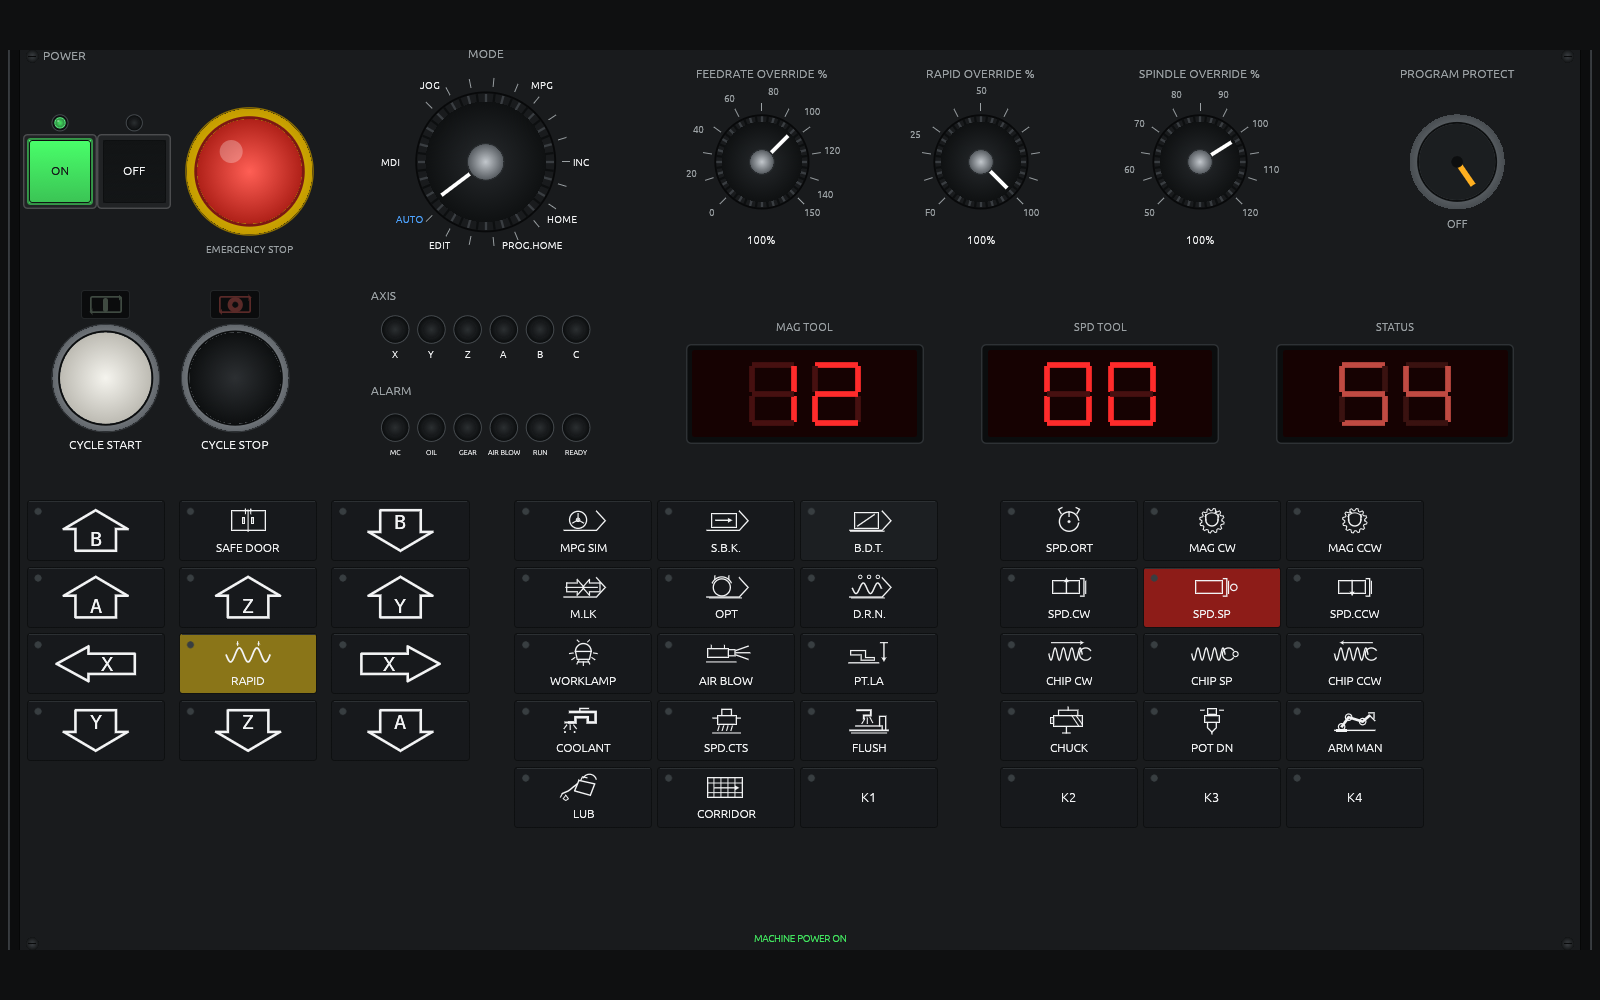
\includegraphics[width=0.86\textwidth]{img/ui/panel.png}};
    \draw[safetyyellow, line width=2pt] ([xshift=1.5cm,yshift=9.6cm]current page.south west) -- ++(9cm,0);
    \node[anchor=north west, text width=17cm, align=left] at ([xshift=1.5cm,yshift=9.2cm]current page.south west) {%
      {\sffamily\bfseries\fontsize{40}{44}\selectfont LiNC}\\[0.6ex]
      {\sffamily\color{safetyyellow}\fontsize{17}{20}\selectfont Operator Manual}\\[1.6ex]
      {\sffamily\color{steel}\small
       LinuxCNC HMI \textbullet{} operator panel \textbullet{} CNC keyboard \textbullet{}
       toolpath \textbullet{} MDI \textbullet{} touch probe \textbullet{} tool table}%
    };
    \node[anchor=south west, text width=16cm, align=left] at ([xshift=1.5cm,yshift=1.2cm]current page.south west) {%
      {\sffamily\color{steel}\small
       End-user documentation for the LiNC controller interface and the panel that
       drives it.\hfill Edition 1.0}%
    };
  \end{tikzpicture}
\end{titlepage}
\pagecolor{white}

\frontmatter
\chapter*{Safety Notice and Disclaimer}
\markboth{Safety Notice and Disclaimer}{}

This manual describes software. The software is not a safety device.

\begin{safetybox}
  A CNC machine is dangerous. The emergency stop, the guards, the door interlocks, the limit
  switches and the machine's own safety circuits are hardware. They must stay functional and
  independent of this software, and they must never be bypassed. No function of LiNC --
  including the network interlock -- is a safety function.
\end{safetybox}

\section*{No warranty}

LiNC is provided \emph{as is}, without warranty of any kind, express or implied, including
the implied warranties of merchantability, fitness for a particular purpose and
non-infringement. No author, contributor or distributor warrants that the software is free
of errors, that it matches the machine it is used on, or that a program, offset, tool value
or probe result is correct.

\section*{No liability}

To the extent permitted by applicable law, no author, contributor or distributor accepts
liability for any damage arising from the use or misuse of this software or from anything
this manual states. This includes, without limitation:

\begin{itemize}
  \item damage to the machine, its tooling, the workpiece, fixtures or other property;
  \item lost production, lost data or the cost of replacement work;
  \item personal injury, up to and including injury to life, body or health.
\end{itemize}

The software cannot see everything the machine does, cannot prevent every programming error,
and cannot replace an operator's judgement. You are responsible for the programs you run, for
the offsets, tool data and limits you set, and for the safe operation of the machine.

\section*{Acceptance}

By installing, commissioning or operating LiNC you accept this notice and the licence terms.
If you do not accept them, do not use the software.

Nothing in this notice excludes or limits liability that cannot be excluded or limited by
applicable law. In particular, liability for intent, for gross negligence, for injury to
life, body or health, and liability under mandatory product liability law remain unaffected.

\section*{Licence}

LiNC is licensed under the GNU General Public Licence, version 2 or later
(\texttt{GPL-2.0-or-later}). The declaration is in \texttt{Cargo.toml}; the packaging record
is in \texttt{debian/copyright}. Sections 11, 12 and 15 to 17 of that licence contain a
warranty and liability disclaimer; this notice states the same for the machine context and
adds the safety warning.

\begin{notebox}
  This notice is not legal advice. If you deploy LiNC commercially, in a regulated
  environment, or in a setting where its failure could injure someone, have the terms
  reviewed before commissioning.
\end{notebox}

\tableofcontents

\mainmatter
\chapter{Introduction}
\label{ch:intro}

LiNC is the operator interface of a LinuxCNC machine. It shows what the machine is
doing, it loads and edits G-code, and it holds the tool, offset and probing pages.
It runs on the control PC as a single program: there is no helper process, no Python
layer and no web service between the screen and the controller.

LiNC is operated from three surfaces, and none of them is a touch screen:

\begin{enumerate}
  \item The \textbf{operator panel} -- power, emergency stop, mode selector, override
        knobs, jog keys, cycle keys and the machine function keys. This is where the
        machine is controlled.
  \item The \textbf{CNC keyboard} -- navigation, G-code entry, MDI, tool and offset
        values, file handling. Every action on the screen has a key.
  \item The \textbf{screen} -- readouts, the toolpath, the program, the tables and the
        diagnostics. It reports; it does not control motion.
\end{enumerate}

The layout and the key handling follow the conventions of an industrial machine
controller, so an operator who knows a conventional control can work without learning
a new interaction model. A mouse is not required, and a touch screen is not required.

The panel and the interface can also run on one computer without a machine cabinet: the
\emph{simulated panel} is a second window that carries the same keys, knobs, lamps and
displays, and publishes the same interface to the controller. On a machine without a
physical panel it stands in for one; a touch screen or a mouse then works as a
replacement for the panel keys. It is a replacement for a panel, not a second way to
drive the machine.

Because the machine controls stay off the screen, the screen is free for machine state.
The digital readout, the toolpath, the program listing, the modal codes and the servo
load are visible at the same time, which is what supervising a running job needs.

\shot{img/ui/machine.png}{The Machine page with a program loaded: readout, toolpath,
program listing, feed and spindle, servo load.}{fig:intro-machine}

\section{What makes LiNC different}

\begin{description}[font=\normalfont\sffamily\bfseries, leftmargin=4.6cm, style=nextline]
  \item[The panel stays the panel] There is no on-screen jog, no on-screen cycle start,
        no override slider and no software emergency stop. A second copy of a control
        drifts out of agreement with the hardware, so there is no second copy.
  \item[MDI is a working area] The MDI pane keeps the blocks you have issued and draws
        the block you are typing on the toolpath before it is sent. A block that would
        leave the machine's travel is refused by name.
  \item[The toolpath explains itself] The loaded program, the live tool trail, the
        machine envelope and the part bounds are separate layers with separate colours.
        Anything outside the machine's travel is drawn solid red.
  \item[Tool changes without MDI] Select a row in the tool table and press \keycap{T}.
        The change and its length compensation are issued for you.
  \item[The editor checks the work] The Program page is a G-code editor with syntax
        highlighting, undo, redo and a live preview. An edit reaches the drawing only
        after it parses.
  \item[Probing is guided] Categories, illustrated operations, parameters and results,
        using the Probe Basic G-code routines that ship with LiNC.
  \item[Help is on the machine] A searchable G-code reference, offline, readable while a
        program runs.
  \item[The network can be taken away] When a program is loaded or MDI is selected, LiNC
        can hold the machine's external network link down, so WiFi latency cannot reach
        the realtime path. \chordtwo{Ctrl}{U} unloads the program and releases it.
\end{description}

\section{What the software will not do}

These are design rules, not preferences. Each one exists so that the screen and the
machine cannot disagree.

\begin{itemize}
  \item It will not jog, home, start the spindle, change coolant or start a cycle.
        Those are panel actions, wired through the machine's HAL.
  \item It will not write an arbitrary HAL pin. It writes seven declared outputs, and
        the list is fixed in the profile and in the program.
  \item It will not save G-code, write a table, import a file or apply a probe result
        while the panel's \pbtn{PROGRAM PROTECT} switch is on.
  \item It will not home an axis. It reports homing and explains the sequence.
  \item It will not guess. A stale or invalid panel state is shown as unknown and fails
        closed.
\end{itemize}

\section{How to read this manual}

\begin{description}[font=\normalfont\sffamily\bfseries, leftmargin=4.2cm, style=nextline]
  \item[Chapter \ref{ch:power}] Powering up and down, emergency stop, protect switch,
        the network interlock.
  \item[Chapter \ref{ch:panel}] Every control on the operator panel.
  \item[Chapter \ref{ch:keyboard}] The keyboard, the navigation column and every
        shortcut.
  \item[Chapter \ref{ch:screen}] The fixed shell: top bar, bottom bar, banners,
        messages.
  \item[Chapter \ref{ch:modes}] Panel modes, jogging, homing and program zero.
  \item[Chapter \ref{ch:running}] Loading, checking and running a program.
  \item[Chapter \ref{ch:mdi}] MDI and the G-code editor.
  \item[Chapter \ref{ch:tools}] Tool table, tool changes, offsets.
  \item[Chapter \ref{ch:probing}] Touch probing.
  \item[Chapter \ref{ch:diagnostics}] Diagnostics, logs and troubleshooting.
  \item[Chapter \ref{ch:quickref}] Key tables and reference data.
\end{description}

Boxes used throughout the manual:

\begin{safetybox}
  Instructions that prevent injury. Read them before operating the machine.
\end{safetybox}
\begin{cautionbox}
  Instructions that prevent damage to the machine, the tooling or the workpiece.
\end{cautionbox}
\begin{notebox}
  Context and cross references.
\end{notebox}
\begin{tipbox}
  Practical hints from the shop floor.
\end{tipbox}

\section{Notation}

Panel keys are drawn as \pbtn{CYCLE START}, screen actions and labels as \sbtn{SAVE},
keyboard keys as \keycap{F6} and key chords as \chordtwo{Ctrl}{S}. Lit panel
lamps are drawn as \ledlit{ledgreen} (lit) against \leddim{ledgreen} (dark). A state
word the screen paints is written as \state{NOT HOMED}.

Positions on the millimetre machine are in millimetres, speeds in millimetres per
minute, spindle speed in revolutions per minute. A lathe profile shows X in the
radius or diameter convention its INI selects.

\section{Terms used in this manual}

\begin{longtable}{L{3.4cm}L{9.6cm}}
  \toprule
  \textbf{Term} & \textbf{Meaning} \\
  \midrule
  \endhead
  HMI & Human-machine interface: this program. \\
  Panel & The operator panel, physical or simulated. It owns the machine controls. \\
  Controller & LinuxCNC: task, motion and I/O. It is authoritative for machine state. \\
  Task mode & LinuxCNC's own mode (MANUAL, MDI, AUTO). The panel requests it; LiNC
              displays it. \\
  Panel mode & The position of the mode selector on the panel. LiNC reads it as one-hot
              signals and fails closed if it is invalid. \\
  WCS & Work coordinate system, \texttt{G54} to \texttt{G59.3}. \\
  DTG & Distance to go: how far the tool still has to move. \\
  MDI & Manual data input: one block, issued immediately. \\
  HAL & LinuxCNC's hardware abstraction layer. \\
  Protect & The panel's \pbtn{PROGRAM PROTECT} key switch. It locks every write. \\
  Interlock & The rule that holds the external network link down while the machine can
              move. \\
  \bottomrule
\end{longtable}

\chapter{Power, Emergency Stop and Safety}
\label{ch:power}

The machine is switched on and off at the panel. LiNC follows: it shows the power and
emergency-stop state on every page, and it blocks machine-modifying actions while either
of them forbids motion.

\section{The power controls}

\begin{figure}[H]
  \centering
  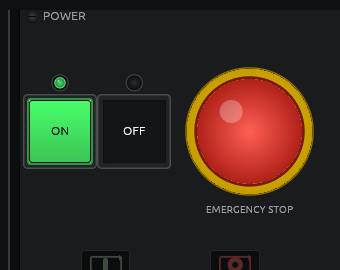
\includegraphics[width=0.42\textwidth]{img/crops/power.png}
  \caption{The power group: \textbf{ON} (lit green when machine power is on),
           \textbf{OFF}, and the emergency stop mushroom.}
  \label{fig:power}
\end{figure}

\begin{description}[font=\normalfont\sffamily\bfseries, leftmargin=3.4cm, style=nextline]
  \item[\pbtn{ON}] Switches machine power on and requests \emph{machine on} in the
        controller. Drives and outputs are enabled. The lamp in the key lights green.
  \item[\pbtn{OFF}] Switches machine power off. LiNC ends its session when the
        controller reports that machine power has dropped.
  \item[EMERGENCY STOP] The red mushroom. It latches when pressed and is released by
        turning it clockwise. See section~\ref{sec:estop}.
\end{description}

The simulator starts in the state a real cabinet is found in: emergency stop latched and
power off. Nothing moves until the mushroom is released and \pbtn{ON} is pressed. This is
deliberate: the power-up sequence is part of the training.

\section{Switching on}

\begin{enumerate}
  \item Check that the work area is clear, the guards are closed and no tool or clamp is
        left on the table.
  \item Release the emergency stop: turn the red mushroom clockwise until it pops out.
  \item Press \pbtn{ON}. The controller enables the drives.
  \item Wait for the panel's \ledlit{leddamber} \state{READY} lamp and for the interface
        to show \state{MACHINE ON} in the bottom bar.
  \item Home the axes (chapter~\ref{ch:modes}). \state{NOT HOMED} in the bottom bar means
        the controller has no valid reference, and no program will start.
  \item Load the program (chapter~\ref{ch:running}), check it, then run it from the panel.
\end{enumerate}

\begin{notebox}
  LiNC does not power the machine on and does not home it. Both are panel actions, wired
  to the controller through the machine's HAL. LiNC reports their state.
\end{notebox}

\section{Emergency stop}
\label{sec:estop}

\begin{safetybox}
  The emergency stop stops all axis motion, the spindle and the coolant immediately.
  Keep it reachable. Never bypass it, and never work around a machine that will not
  leave the emergency-stop state.
\end{safetybox}

Behaviour on this controller:

\begin{itemize}
  \item \textbf{Pressing} the mushroom latches the panel input. The controller enters
        emergency stop, drives are disabled and motion stops. LiNC shows the red banner
        \state{EMERGENCY STOP ACTIVE — MOTION AND MACHINE ACTIONS BLOCKED} on every page,
        and the bottom bar reads \state{E-STOP ACTIVE}.
  \item \textbf{Releasing} the mushroom clears the latch and asks the controller to leave
        emergency stop. It does \emph{not} switch machine power on: that is a separate
        \pbtn{ON} press. This separation is deliberate, so releasing the mushroom cannot
        start the machine.
  \item After a release, press \pbtn{ON} again if power dropped, check \state{READY}, and
        check the homing state before continuing.
\end{itemize}

\begin{cautionbox}
  An emergency stop interrupts the program mid-block. Before restarting, inspect the tool
  position and the remaining path. Use single block and a reduced feed override for the
  first blocks after recovery.
\end{cautionbox}

\section{Switching off}

\begin{enumerate}
  \item Finish or stop the running program (\pbtn{CYCLE STOP} on the panel).
  \item Unload the program with \chordtwo{Ctrl}{U} on the Program page if you are
        finished with it (section~\ref{sec:unload}).
  \item Press \pbtn{OFF}. The controller shuts down and LiNC ends its session.
\end{enumerate}

\begin{cautionbox}
  Do not cut the main disconnect while a program is running. Use \pbtn{OFF} first, so the
  controller can stop in a defined state.
\end{cautionbox}

LiNC refuses a normal quit (\chordtwo{Ctrl}{Q}) while a program is running or an
axis is moving. Losing machine power is the one case where the session ends regardless,
because the controller is going away anyway.

\section{Program protect}

\begin{figure}[H]
  \centering
  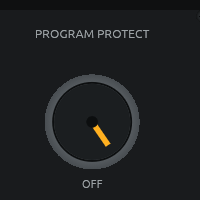
\includegraphics[width=0.24\textwidth]{img/crops/protect.png}
  \caption{The \textbf{PROGRAM PROTECT} key switch. \texttt{OFF} is the working position;
           \texttt{ON} locks every write.}
  \label{fig:protect}
\end{figure}

The panel's key switch is authoritative. While it is on, LiNC cannot:

\begin{itemize}
  \item edit the program buffer or save it,
  \item write an offset, a tool row or a tool length,
  \item copy or import a file into the program directory,
  \item apply a probe result to a work offset.
\end{itemize}

The screen shows the banner \state{PROTECT ON — EDITING LOCKED} on the pages that write,
and the field \state{PROTECT ON} in the bottom bar. Reading, loading and running a program
remain possible: protect blocks writing, not viewing.

\begin{notebox}
  Protect fails closed. If the switch state is unknown or the panel data is stale, LiNC
  treats protect as \emph{on}. Every write checks it again in the backend; a value the
  screen sampled earlier is not enough.
\end{notebox}

Unsaved edits are not thrown away when protect is switched on. The buffer stays, keeps
its dirty marker and becomes read-only until the switch returns to \texttt{OFF}.

\section{Limits override}

If an axis stands on a limit switch, the panel's jog keys are refused. The keyboard chord
\chordthree{Ctrl}{Shift}{O} toggles the controller's limit-switch override so
the axis can be jogged off the switch.

\begin{cautionbox}
  While the override is on, the limit switches are ignored and the machine can be driven
  past them. The screen shows a blinking \state{LIMITS OVERRIDE ON} in the bottom bar and
  the banner \state{LIMITS OVERRIDE ACTIVE — LIMIT SWITCHES ARE IGNORED}, but neither
  stops the machine. Jog off the switch, then switch the override off again.
\end{cautionbox}

\section{Panel offline and invalid mode}

LiNC reads the panel through the panel service. Two failures are shown as banners and
both fail closed:

\begin{description}[font=\normalfont\sffamily\bfseries, leftmargin=4.2cm, style=nextline]
  \item[\state{PANEL OFFLINE}] No current panel data. Machine-modifying actions are
        blocked, and the top bar's \state{PANEL} dot turns red.
  \item[\state{PANEL MODE INVALID}] The mode selector reports zero or more than one
        position. LiNC does not guess: the mode reads \state{UNKNOWN} and mode-dependent
        actions are refused until a valid position arrives.
\end{description}

The hardware emergency stop is independent of both. It works even when the panel service
is down, because it is wired in the machine's HAL.

\section{The external link interlock}
\label{sec:interlock}

On a machine whose only external network link is WiFi, LiNC can hold that link down while
the machine is able to move. WiFi association, driver interrupts and packet bursts all
cost realtime, and none of them are needed while a program runs.

\begin{notebox}
  The interlock only ever touches the external link named in the profile. The machine's
  internal fieldbus is never touched.
\end{notebox}

\textbf{When it is armed.} The link is held down while a program is loaded or the panel is
in \texttt{MDI}. It is released when nothing is loaded and no MDI block is being set up.
This is arm-on-intent, not arm-on-motion: a loaded program that is paused still holds the
link down, because it can be resumed.

\textbf{The \state{NET} field.} The top bar always shows the link state:

\begin{center}
\begin{tabular}{lll}
  \toprule
  \textbf{Value} & \textbf{Colour} & \textbf{Meaning} \\
  \midrule
  \state{DOWN} & green & Link down. This is the state the interlock wants while armed. \\
  \state{UP}   & muted & Link up, no program motion. Normal while setting up. \\
  \state{UP}   & amber & Link up \emph{and} program motion. The one state to look at. \\
  \state{MEAS} & accent & A link measurement is running. \\
  \state{?}    & amber & State unknown or stale. Fails closed. \\
  \state{OFF}  & muted & No interlock configured in this profile. \\
  \bottomrule
\end{tabular}
\end{center}

Amber is reserved for program motion on purpose. Jogging and homing keep the link up by
design, and colouring every setup jog amber would train the operator to ignore the one
colour that matters.

\textbf{Releasing the link.} Press \chordtwo{Ctrl}{U} on the Program page. LiNC
closes the program at the controller, resets the interpreter, re-reads the program name and
only then reports success. The \state{NET} field returns to \state{UP} within a few
seconds, after the radio has associated and a default route exists. A toast says
\state{UNLOAD REQUESTED — WATCH NET}.

\begin{cautionbox}
  Leaving a program loaded keeps the link down, and the link is the only remote way into
  the machine. If you need remote access while nothing is being cut, unload the program
  first. Profiles that must keep the link up can set \texttt{keep\_up = true} in
  \texttt{[network]}.
\end{cautionbox}

If the link is up while a program is loaded, commands that would run or change the program
are refused with \state{NETWORK BUSY} rather than being sent.

\section{Probe trip}

If the probe input rises during a move that is not a probe, the controller aborts the move
and reports an operator error. LiNC treats this as a latched fault, not a passing message:

\begin{itemize}
  \item A red banner carries the controller's own text on every page, for example
        \state{PROBE TRIPPED — … — MACHINE SWITCHED OFF. MOTION AND MDI BLOCKED. RESET
        (ESC) TO CLEAR.}
  \item The machine is switched off through \halpin{linc.machine-off}, so the panel cannot
        jog into the probe either. One exception exists: a trip raised with the program
        paused and nothing moving leaves the machine on, because nothing had to be stopped.
  \item MDI, probe, tool-change, jog-parameter and table writes fail closed until the trip
        is cleared.
  \item \keycap{Esc} (or the banner's \sbtn{RESET}) clears it, from any page. That sends the
        controller reset which clears the motion error. Re-powering afterwards needs a fresh
        \pbtn{ON}.
\end{itemize}

\section{Safety rules, in short}

The safety and liability disclaimer that applies to this software is printed at the front
of this manual, before the contents.

\begin{safetybox}
  \begin{itemize}
    \item The panel is the only place machine motion starts. Do not look for a jog or a
          cycle start on the screen.
    \item Release the emergency stop, then press \pbtn{ON}: two separate actions.
    \item Never leave the machine in limits override.
    \item Never run a program that shows red path outside the machine envelope without
          knowing why.
    \item Unload the program before relying on the network link.
  \end{itemize}
\end{safetybox}

\chapter{The Operator Panel}
\label{ch:panel}

The operator panel is the machine's control surface. Every action that moves the machine,
changes the spindle or changes an override starts here. LiNC reads the panel and shows what
it is doing; it never sends those commands.

The panel runs as its own process (\texttt{linc-panel}) and owns the panel link. It
publishes a fixed set of button, lamp, display and override signals to the controller's
HAL, named \halpin{cnc\_panel.*}. The interface reads the same signals. A crash of the
interface therefore does not take the panel away, and the interface never opens the panel
port.

\begin{notebox}
  The interface cannot write a \halpin{cnc\_panel.*} pin. It writes only its own seven
  declared outputs, and \halpin{net-safe} is the only one that reaches machine logic.
\end{notebox}

\shot{img/ui/panel.png}{The simulated operator panel, mill face. A physical panel carries
the same groups; the machine builder decides the exact legends of the machine function
keys.}{fig:panel}

\section{Power and emergency stop}

The power group and the emergency stop are described in chapter~\ref{ch:power}. The panel
is where they are pressed; the screen only reports them.

\section{The mode selector}

\begin{figure}[H]
  \centering
  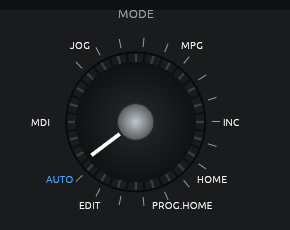
\includegraphics[width=0.44\textwidth]{img/crops/mode.png}
  \caption{The \textbf{MODE} selector. Its eight steady positions are read as one-hot
           signals: exactly one position must be active.}
  \label{fig:mode}
\end{figure}

The selector is read as a steady position, not as pulses. Zero or several active positions
is a fault: LiNC shows \state{PANEL MODE INVALID} and refuses mode-dependent actions.

\begin{longtable}{L{2.5cm}L{4.6cm}L{5.9cm}}
  \toprule
  \textbf{Position} & \textbf{Panel / controller} & \textbf{What LiNC does} \\
  \midrule
  \endhead
  EDIT & Manual mode, editing allowed & Opens Program in the \sbtn{CODE} layout and focuses
         the editor. Saving is allowed only here. \\
  AUTO & Automatic mode & Brings the Machine page forward. Cycle start then belongs to the
         panel. \\
  MDI  & Manual data input & Opens the Machine page with the MDI pane in place of the program
         card. \keycap{Enter} issues the block. \\
  JOG  & Manual mode, continuous jog & Opens the Manual page: live toolpath, coordinates,
         jog context. \\
  INC  & Manual mode, step jog & Same page, with the increment row. The steps come from the
         machine INI. \\
  MPG  & Manual mode, handwheel & Same page; the handwheel selects its own step. \\
  HOME & Manual mode, homing & Opens the Homing page with the machine position and the homing
         state of each axis. \\
  PROG.HOME & Manual mode, program zero & Opens the Homing page titled \state{PROGRAM ZERO}. The
         axis keys send the program-zero blocks, not jogs. \\
  \bottomrule
\end{longtable}

\begin{notebox}
  The selector is authoritative for what the panel keys do. LiNC's own page changes are a
  convenience copy of that state; where the two disagree, the panel wins. The top bar shows
  \state{PANEL} and \state{TASK} separately, so a disagreement is visible.
\end{notebox}

\section{The override knobs}

\begin{figure}[H]
  \centering
  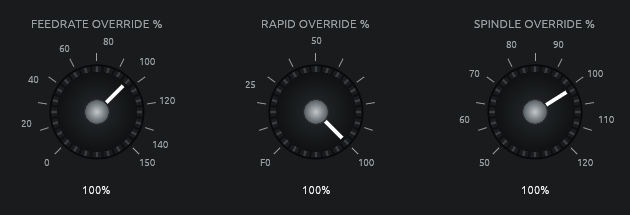
\includegraphics[width=0.86\textwidth]{img/crops/overrides.png}
  \caption{Feedrate, rapid and spindle override. The percentage under each knob is the
           current value; the interface repeats all three in the bottom bar.}
  \label{fig:overrides}
\end{figure}

The three knobs are steady analogue values sampled by the panel service. LiNC displays them
as \state{OVR F100 R100 S100} in the bottom bar, and the Machine page uses the feed and
spindle percentages in its \sbtn{FEED / SPINDLE} card.

\begin{itemize}
  \item \textbf{Feedrate override} scales programmed feed. On the shipped panel it ranges
        from 0 to 150\,\%.
  \item \textbf{Rapid override} scales rapid moves. \texttt{F0} stops rapids.
  \item \textbf{Spindle override} scales the commanded spindle speed. It does not change the
        displayed true speed, which comes from feedback.
\end{itemize}

\begin{cautionbox}
  An override of 0\,\% feed looks like a machine that will not move. Check the knobs before
  diagnosing a fault: the bottom bar always shows them.
\end{cautionbox}

\section{Cycle keys and axis keys}

\begin{figure}[H]
  \centering
  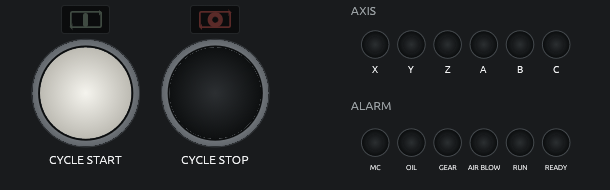
\includegraphics[width=0.77\textwidth]{img/crops/lamps.png}
  \caption{Left: \textbf{CYCLE START} (illuminated white) and \textbf{CYCLE STOP}. Centre: the
           axis lamps. Right: the alarm lamps.}
  \label{fig:cyclekeys}
\end{figure}

\begin{description}[font=\normalfont\sffamily\bfseries, leftmargin=3.1cm, style=nextline]
  \item[\pbtn{CYCLE START}] Starts the loaded program. The controller gates it: machine on,
        no emergency stop, axes homed, interpreter idle, and the panel in AUTO. LiNC does
        not issue it and cannot issue it.
  \item[\pbtn{CYCLE STOP}] Stops the program and stops motion.
  \item[Axis keys] Jog in JOG and INC, home in HOME, and send the program-zero block in
        PROG.HOME, all according to the mode selector and the machine's HAL wiring.
  \item[\pbtn{RAPID}] With an axis key, jogs at rapid rate; in HOME it starts homing all
        axes; in PROG.HOME it sends the all-axes program-zero block.
\end{description}

The axis lamps light for the axes the controller reports. The alarm lamps report machine
conditions (machine ready, run, and the machine's own alarm set). \state{READY} follows
machine power and an idle or paused program.

\section{The displays}

\begin{figure}[H]
  \centering
  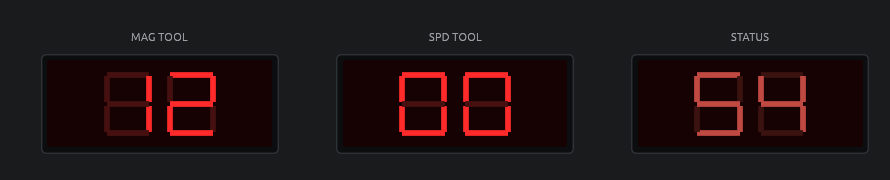
\includegraphics[width=0.95\textwidth]{img/crops/displays.png}
  \caption{The tool displays and the two-digit status display. Here the status display
           shows \texttt{54}, the active work coordinate system.}
  \label{fig:displays}
\end{figure}

\begin{itemize}
  \item \textbf{MAG TOOL} is the tool in the spindle as the controller reports it.
  \item \textbf{SPD TOOL} is the prepared tool, where the machine has a changer.
  \item \textbf{STATUS} shows the active work coordinate system, \texttt{54} to
        \texttt{59}. It shows \texttt{-{}-} when the value is unknown, stale or outside
        those systems, and never a guess.
\end{itemize}

The interface writes \halpin{linc.status-display} and the machine's post-GUI HAL maps it to
the display. This is one of the seven declared outputs.

\section{The machine function keys}

The key matrix carries the machine functions: spindle forward, stop, reverse and orient;
coolant; air blow; chuck; lube; chip conveyor; work lamp; safe door; tool changer and pot
keys; and the four free keys \pbtn{K1} to \pbtn{K4}. Each key is a HAL button; the machine
configuration decides what it switches.

\begin{notebox}
  Only the keys the machine wires do something. A key with no net in the machine's HAL is
  inert, and the simulated panel greys the keys its profile does not wire. Nothing on the
  screen duplicates these functions.
\end{notebox}

\section{The simulated panel}

The simulated panel is a window that speaks the same protocol as a physical panel. It is
used for the simulator, for training and for a machine that has no panel cabinet.

\begin{itemize}
  \item It draws the face the profile selects: mill or lathe, with that face's keys, lamps
        and displays.
  \item It publishes the same \halpin{cnc\_panel.*} signals as the real driver, so the
        interface and the HAL cannot tell the difference.
  \item It starts in the safe state: emergency stop latched, power off.
  \item It runs on a second monitor if you put it there. With no physical panel, a touch
        screen or a mouse can operate it; that makes the pointer a replacement for the
        panel hardware, not a second set of machine controls.
\end{itemize}

The panel window also answers the keyboard, so it can be used without a pointer:

\begin{center}
\begin{tabular}{ll}
  \toprule
  \textbf{Key} & \textbf{Action} \\
  \midrule
  \keycap{P} & Power on (also releases the emergency stop) \\
  \keycap{O} & Power off \\
  \keycap{E} & Press / release the emergency stop \\
  \keycap{R} & Rapid (hold) \\
  \keycap{C} & Cycle start \\
  \keycap{S} & Cycle stop \\
  \keycap{1} \dots \keycap{8} & Mode selector: EDIT, AUTO, MDI, JOG, INC, MPG, HOME, PROG.HOME \\
  \bottomrule
\end{tabular}
\end{center}

\begin{tipbox}
  In a demonstration on one computer, keep the panel window on the second monitor and give
  the interface the first one. The interface's \keycap{F5} to \keycap{F8} keys and the
  panel's number keys act on different windows, so the focus must be where the key belongs.
\end{tipbox}

\chapter{The Keyboard and Navigation}
\label{ch:keyboard}

LiNC is built for a CNC panel keyboard: the keys are labelled with what they do at the
machine, not with the letters a PC keyboard happens to send. A normal PC keyboard works
too, and the profile can name the keys either way: \texttt{[ui] keyboard = "panel"} prints
the panel legends, \texttt{[ui] keyboard = "pc"} adds the keys a PC keyboard sends.

Every action in the interface can be reached from the keyboard. Nothing needs a pointer,
nothing needs a touch, and nothing depends on a \keycap{Tab} key.

\section{The navigation column}

\subsection*{The main layer}

The main layer holds what a program is typed from:

\begin{itemize}
  \item the address letters \texttt{O N G X Y Z F D H M S T P Q R} and all ten digits;
  \item \texttt{ENT} to commit, \texttt{BkSp} to delete, \texttt{Space};
  \item the punctuation a program needs: \texttt{. - / ;} and their shifted forms;
  \item the page and cursor keys, and \texttt{Shift} and \texttt{Ctrl};
  \item the five machine keys \pbtn{MAIN}, \pbtn{FILE}, \pbtn{OFFS}, \pbtn{TOOL}, \pbtn{WIN}
        and \pbtn{ESC}.
\end{itemize}

The letters that are rare in G-code -- \texttt{A B C E I J K L U V W} -- are not on the main
layer. They are the blue legends, reached with \keycap{Shift} or a double tap.

\begin{figure}[H]
  \centering
  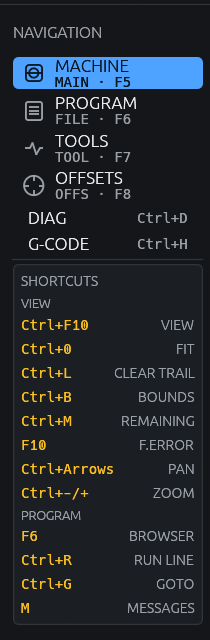
\includegraphics[width=0.24\textwidth]{img/crops/rail.png}
  \caption{The navigation column and the shortcut pane. The shortcut pane lists the keys
           that work on the page in front; it is a reminder, not a set of buttons.}
  \label{fig:rail}
\end{figure}

\begin{longtable}{L{3.4cm}L{2.4cm}L{7.0cm}}
  \toprule
  \textbf{Row} & \textbf{Key} & \textbf{Opens} \\
  \midrule
  \endhead
  \textsf{MACHINE} & \keycap{F5} & The Machine page, or in EDIT/JOG/INC/MPG/HOME the page
        that belongs to the panel mode. \\
  \textsf{PROGRAM} & \keycap{F6} & The Program page. Pressing it again opens the Files
        browser; pressing it in Files brings the program back. \\
  \textsf{TOOLS} & \keycap{F7} & The tool table. \\
  \textsf{OFFSETS} & \keycap{F8} & The work offsets. Pressed again, it moves on to the probe
        tabs, one press per tab, and from the last tab back to Offsets. \\
  \textsf{DIAG} & \chordtwo{Ctrl}{D} & Diagnostics. \\
  \textsf{G-CODE} & \chordtwo{Ctrl}{H} & The G-code help. \\
  \bottomrule
\end{longtable}

The profile may hide rows or change their order, so a machine can ship without the pages it
does not use.

\section{Focus and movement}

The shell has three focus regions: the navigation column, the page, and the page's actions.
The focused element always has a visible ring.

\begin{description}[font=\normalfont\sffamily\bfseries, leftmargin=3.2cm, style=nextline]
  \item[Arrow keys] Move within the current region: rows, table cells, list entries, chips.
  \item[\keycap{Enter}] Activates: open a folder, load a program, commit a cell, issue an MDI
        block, run the highlighted routine.
  \item[\keycap{Esc}] Goes back: closes a dialog, leaves the help article, cancels an edit.
        On any page while a program is active it resets the program.
  \item[\keycap{Home}] / \keycap{End} First and last entry of a list. Inside a text field
        they move to the start and end of the line.
  \item[\keycap{PgUp}] / \keycap{PgDn} A screenful in a list or a read-only program; on
        Diagnostics and the probe tabs, the next tab.
\end{description}

A text field that holds the keyboard keeps the page keys for itself: inside the editor,
\keycap{PgUp} moves the cursor rather than the page.

\section{Keys that work everywhere}

\begin{longtable}{L{4.7cm}L{8.1cm}}
  \toprule
  \textbf{Keys} & \textbf{Action} \\
  \midrule
  \endhead
  \keycap{F5} \dots \keycap{F8} & Navigation, as in the table above. \\
  \chordtwo{Ctrl}{D} & Diagnostics. \\
  \chordtwo{Ctrl}{H} & G-code help. \\
  \keycap{M} & The full-screen messages dialog. \\
  \keycap{Esc} & Back, cancel, or reset the program when one is active. \\
  \chordtwo{Ctrl}{Q} & Quit. Refused while a program runs or an axis moves. \\
  \chordtwo{Ctrl}{O} & Open the Files browser, from any page except Program, where
        \keycap{F6} does it. \\
  \chordtwo{Ctrl}{S} & Save the editor buffer. \\
  \chordtwo{Ctrl}{Z} / \chordtwo{Ctrl}{Y} & Undo / redo in the editor. \\
  \chordtwo{Ctrl}{F} & Search the G-code help (Help page only). \\
  \chordthree{Ctrl}{Shift}{O} & Toggle the limit-switch override. \\
  \bottomrule
\end{longtable}

\begin{cautionbox}
  \chordtwo{Ctrl}{Q} ends the session. It is refused while the machine is busy on
  purpose: a quit prompt in the middle of a cut is a dialog in the way.
\end{cautionbox}

\section{Keys for the toolpath}

Every page that draws a toolpath answers the same view keys, so a view command learned on
one page works on the next.

\begin{longtable}{L{4.7cm}L{8.1cm}}
  \toprule
  \textbf{Keys} & \textbf{Action} \\
  \midrule
  \endhead
  \chordtwo{Ctrl}{F10} & Cycle the view: ISO, X, Y, Z. A lathe toggles ISO and its XZ
        view. \\
  \chordtwo{Ctrl}{0} & Fit the drawing to the page. \\
  \chordtwo{Ctrl}{L} & Clear the live tool trail only. \\
  \chordtwo{Ctrl}{B} & Cycle the bounds: program dimensions, machine envelope, program
        box, off. \\
  \chordtwo{Ctrl}{M} & REMAINING: show only what is still to run. \\
  \keycap{Ctrl}+arrows & Pan the view. \\
  \chordtwo{Ctrl}{+} / \chordtwo{Ctrl}{-} & Zoom in / out. \\
  \bottomrule
\end{longtable}

The pointer does the same: dragging pans, the wheel zooms, a middle-drag orbits in 3D, and a
double click returns to the default isometric view. On the keyboard, \chordtwo{Ctrl}{F10}
and \chordtwo{Ctrl}{0} cover the two commands that matter most.

\section{Keys for programs and the editor}

\begin{longtable}{L{4.7cm}L{8.1cm}}
  \toprule
  \textbf{Keys} & \textbf{Action} \\
  \midrule
  \endhead
  \chordtwo{Ctrl}{R} & RUN FROM LINE: start the loaded program at the selected line. \\
  \chordtwo{Ctrl}{G} & GO TO LINE: ask for a line number and move the view there. \\
  \chordtwo{Ctrl}{U} & UNLOAD: close the program and release the network interlock. \\
  \keycap{F10} & Toggle the Program layout: SPLIT and CODE. \\
  \chordtwo{Ctrl}{\textuparrow} / \chordtwo{Ctrl}{\textdownarrow} & Move the selected line up or down in
        the editor. \\
  \chordtwo{Ctrl}{\textleftarrow} / \chordtwo{Ctrl}{\textrightarrow} & Move by word in the editor and the
        MDI input. \\
  \chordtwo{Ctrl}{A} / \keycap{C} / \keycap{X} / \keycap{V} & Select all, copy, cut,
        paste in the editor. \\
  \chordtwo{Ctrl}{K} & Delete the current line in the editor. \\
  \chordtwo{Ctrl}{D} & Duplicate the current line in the editor. It shadows the
        Diagnostics key while the editor has the keyboard. \\
  \bottomrule
\end{longtable}

\begin{notebox}
  \chordtwo{Ctrl}{R} has three page-local meanings: run from line on Program, run the
  selected block in the MDI pane, and refresh the listing in Files. The shortcut pane always
  shows the one that applies now.
\end{notebox}

\section{Reading the shortcut pane}

The pane under the navigation column lists the page's own keys in groups: \state{VIEW},
\state{PROGRAM}, \state{BROWSE}, \state{FILE}, \state{MEDIA}, \state{LOG VIEW},
\state{PROBE KEYS} and so on. Each line is a key or chord on the left and the action it
performs on the right. The list changes with the page and with the state: while the MDI pane
is up it lists the MDI keys instead of the program keys, and while the editor holds the
keyboard it lists the line-move chords.

When the pane shows nothing, the page has no page-local keys. The global keys above still
work.

\section{Dialogs}

A dialog owns the keyboard while it is open. \keycap{Enter} confirms, \keycap{Esc} cancels,
the arrows move between its buttons or fields, and nothing behind it reacts to a key. The
messages dialog scrolls with \keycap{PgUp}/\keycap{PgDn} and closes with \keycap{Enter} or
\keycap{Esc}.

The unsaved-changes dialog has no third option: save, discard, or cancel the action that
would have thrown the buffer away. Saving is greyed out when a condition blocks it, and the
dialog names the condition.

\clearpage
\section{The CNC keyboard}
\label{sec:cnckeyboard}

The machine keyboard is a 48-key USB keyboard with per-key RGB backlight. Its layout is the
industrial-controller layout: the letters and digits a G-code program is written from sit on
the main layer, and everything else is reached with \keycap{Shift} or by tapping a key twice.
The bottom row carries the navigation keys, so the whole interface is within one hand's reach.

\begin{figure}[H]
  \centering
  \begin{tikzpicture}
    % row 0
    \kbkey{0}{0}{O}{A}   \kbkey{1}{0}{N}{B}   \kbkey{2}{0}{G}{C}
    \kbkey{3}{0}{7}{\%}  \kbkey{4}{0}{8}{@}   \kbkey{5}{0}{9}{\#}
    % row 1
    \kbkey{0}{1}{X}{U}   \kbkey{1}{1}{Y}{V}   \kbkey{2}{1}{Z}{W}
    \kbkey{3}{1}{4}{\$}  \kbkey{4}{1}{5}{:}   \kbkey{5}{1}{6}{=}
    % row 2
    \kbkey{0}{2}{F}{E}   \kbkey{1}{2}{D}{L}   \kbkey{2}{2}{H}{[}
    \kbkey{3}{2}{1}{]}   \kbkey{4}{2}{2}{<}   \kbkey{5}{2}{3}{>}
    % row 3
    \kbkey{0}{3}{M}{I}   \kbkey{1}{3}{S}{J}   \kbkey{2}{3}{T}{K}
    \kbkey{3}{3}{.}{,}   \kbkey{4}{3}{0}{\textbackslash} \kbkey{5}{3}{-}{+}
    % row 4
    \kbkey{0}{4}{P}{(}   \kbkey{1}{4}{Q}{)}   \kbkey{2}{4}{R}{\&}
    \kbkey{3}{4}{/}{*}   \kbkey{4}{4}{;}{\_}  \kbkey{5}{4}{ENT}{m1}
    % row 5
    \kbkey{0}{5}{PgUp}{} \kbkey{1}{5}{Home}{} \kbkey{2}{5}{\textuparrow}{m\,\textuparrow}
    \kbkey{3}{5}{End}{}  \kbkey{4}{5}{Space}{} \kbkey{5}{5}{BkSp}{tetris}
    % row 6
    \kbkey{0}{6}{PgDn}{} \kbkey{1}{6}{\textleftarrow}{m\,\textleftarrow}
    \kbkey{2}{6}{\textdownarrow}{m\,\textdownarrow}
    \kbkey{3}{6}{\textrightarrow}{m\,\textrightarrow}
    \kbkey{4}{6}{SHIFT}{} \kbkey{5}{6}{Ctrl}{}
    % row 7
    \kbkey{0}{7}{MAIN}{F5} \kbkey{1}{7}{FILE}{F6} \kbkey{2}{7}{OFFS}{F8}
    \kbkey{3}{7}{TOOL}{F7} \kbkey{4}{7}{WIN}{F10} \kbkey{5}{7}{ESC}{}
  \end{tikzpicture}
  \caption{Keyboard layout. Centre: the main layer. Small blue legends: the shift and
           double-tap layer (\texttt{m} = mouse key).}
  \label{fig:keyboard}
\end{figure}


\subsection*{Shift and double tap}

\begin{description}[font=\normalfont\sffamily\bfseries, leftmargin=2.6cm, style=nextline]
  \item[\keycap{Shift}] Hold it, then press the key: the blue legend is sent. The dual-layer
        keys glow brighter blue while Shift is held.
  \item[Double tap] Tap the same key twice within 0.3\,s. The first character is erased and
        the blue legend is written instead: \keycap{O}\,\keycap{O} writes \texttt{A},
        \keycap{7}\,\keycap{7} writes \texttt{\%}, \keycap{F}\,\keycap{F} writes \texttt{E}.
\end{description}

Letters are transmitted lowercase. G-code words are not case sensitive in LinuxCNC, so
lowercase letters are fine in MDI and in the editor.

A handful of secondary legends are not characters: the arrow keys become a mouse
(\texttt{m\,$\uparrow$} moves the pointer, \texttt{m1} on \pbtn{ENT} clicks), and a double tap
on \pbtn{BkSp} starts a small game (section~\ref{sec:kbtips}).

\subsection*{Backlight}

An idle key glows dim blue. A pressed key lights \textbf{white}; when the press produces a
blue legend, it lights \textbf{yellow}. The backlight is the state display of the keyboard:
if a key stays yellow after it was pressed, the secondary layer was sent.

\subsection*{The machine keys}

\begin{longtable}{L{3.4cm}L{2.6cm}L{7.6cm}}
  \toprule
  \textbf{Legend} & \textbf{Sends} & \textbf{Opens} \\
  \midrule
  \endhead
  \pbtn{MAIN} & \keycap{F5} & The Machine page, or in EDIT, JOG, INC, MPG or HOME the page that
        belongs to the panel mode. \\
  \pbtn{FILE} & \keycap{F6} & Program. Pressed again, Files; in Files, back to Program. \\
  \pbtn{TOOL} & \keycap{F7} & Tools. \\
  \pbtn{OFFS} & \keycap{F8} & Offsets. Pressed again, the probe tabs. \\
  \pbtn{WIN} & \keycap{F10} & SPLIT / CODE on Program. With \keycap{Ctrl}, cycle the toolpath
        view. \\
  \pbtn{ESC} & \keycap{Esc} & Back, cancel, or reset the program when one is active. \\
  \bottomrule
\end{longtable}

The interface does not depend on the printed letters. It depends on the keys these legends
send, which is why a normal PC keyboard works as well: \keycap{F5} to \keycap{F8},
\keycap{F10} and \keycap{Esc} are the same keys.

\subsection*{Typing in the editor}

The keyboard has no \keycap{Tab} and no \keycap{Delete}. Write spaces, delete with
\keycap{BkSp}, and use \chordtwo{Ctrl}{A}, \chordtwo{Ctrl}{C}, \chordtwo{Ctrl}{X} and
\chordtwo{Ctrl}{V} to select, copy, cut and paste. Line-based editing -- duplicate a line,
delete a line, move a line -- is on \chordtwo{Ctrl}{D}, \chordtwo{Ctrl}{K} and the
\chordtwo{Ctrl}{arrows} chords, because those do not need a pointer.

\subsection*{Service combinations}
\label{sec:kbtips}

\begin{cautionbox}
  \keycap{Shift}+\pbtn{MAIN} puts the keyboard into its firmware bootloader, and
  \keycap{Shift}+\pbtn{ESC} quits the user interface. Both are service functions. Do not press
  them during machining.
\end{cautionbox}

\begin{tipbox}
  Hold \keycap{Shift}+\pbtn{BkSp} for three seconds and the LED matrix plays a small game
  (arrows steer, hold again to quit). A progress bar on the bottom row shows the activation.
  Best used during coffee, not during cutting.
\end{tipbox}

\begin{notebox}
  If a key seems dead, look at the shortcut pane first: the key may be page-local and not
  belong to the page in front. \chordtwo{Ctrl}{D} inside the editor is a good example -- it
  duplicates a line there, and reaches Diagnostics everywhere else.
\end{notebox}

\chapter{The Screen}
\label{ch:screen}

The screen has a fixed shell. Every page keeps the same frame, so the numbers an operator
watches are always in the same place.

\begin{figure}[H]
  \centering
  
\includegraphics[width=\textwidth]{img/crops/topbar.png}
  \caption{The top bar. Left: program identity and the panel and task modes. Centre: the
           machine metrics. Right: panel link, message and alarm counters, frame rate and
           clock.}
  \label{fig:topbar}
\end{figure}

\shot{img/ui/machine.png}{The Machine page. The shell around it -- top bar, navigation
column, shortcut pane, bottom bar -- is present on every page.}{fig:screen-main}

\section{The top bar}

\begin{description}[font=\normalfont\sffamily\bfseries, leftmargin=3.0cm, style=nextline]
  \item[LiNC] The program name, and a \state{SIM} badge when the session is a simulation.
        The machine name comes from the profile.
  \item[PANEL] The panel's mode selector position. Accent-coloured when valid, red when the
        mode is unknown or invalid.
  \item[TASK] The controller's own task mode. It follows the panel, but it is the
        controller that decides.
  \item[PROGRAM] The loaded program's file name, or \state{-{}-} when none is loaded.
  \item[STATE] \state{IDLE}, \state{RUNNING} or \state{PAUSED}, with the colour that
        belongs to it.
  \item[TOOL] The tool in the spindle as the controller reports it.
  \item[SPINDLE] The measured spindle speed in revolutions per minute.
  \item[FEED] The programmed feed rate.
  \item[WORK] The active work coordinate system.
  \item[NET] The external link state (chapter~\ref{ch:power}).
\end{description}

On the right: the \state{PANEL} status dot with its link state, the message and alarm
counters, the render rate and the clock. A frame rate below 30 is amber: it is the first
number to ask about when the interface feels slow.

\begin{notebox}
  The counters are read-only. \state{MSG} counts the entries in the message log, \state{ALARM}
  counts the errors among them. Neither is a button.
\end{notebox}

\section{The bottom bar}

\begin{figure}[H]
  \centering
  
\includegraphics[width=\textwidth]{img/crops/bottombar.png}
  \caption{The bottom bar: machine state on the left in the flow, the read-only safety and
           override group on the right.}
  \label{fig:bottombar}
\end{figure}

Fields appear only when they have something to say:

\begin{longtable}{L{3.6cm}L{9.2cm}}
  \toprule
  \textbf{Field} & \textbf{Meaning} \\
  \midrule
  \endhead
  \state{LN 12/340 34\%} & The executing line, the line count and the program progress. \\
  \state{HOMED} & Every axis is homed. A partly homed machine says \state{HOMED X} and
        names the axes it already trusts. \\
  \state{NOT HOMED} & No axis is homed. Motion commands are refused. \\
  \state{LIMIT X} & A limit switch is held. Motion is blocked and the axis is named. \\
  \state{TC T7 PENDING} & A manual tool change is waiting for confirmation. \\
  \state{DTG Z +1.234} & Distance still to go on the axis that is moving. On the Program page
        this becomes a full coordinate line for every axis. \\
  \state{E-STOP ACTIVE} / \state{E-STOP OK} / \state{E-STOP ?} & The emergency-stop state, or
        a question mark when the data is stale. \\
  \state{MACHINE ON} / \state{MACHINE OFF} & Machine power. \state{MACHINE OFF} blinks: it is
        a fault, not a normal idle. \\
  \state{PROBE READY} / \state{PROBE TRIPPED} / \state{PROBE ?} & The wired probe input. The
        field is drawn only while the probe tool is in the spindle. \\
  \state{PROTECT ON} & The panel's program-protect switch is on. \\
  \state{OVR F100 R100 S100} & Feed, rapid and spindle override. \\
  \state{LIMITS OVERRIDE ON} & Blinking. The limit switches are being ignored. \\
  \state{AUTO} & The panel mode, repeated here for a glance. \\
  \bottomrule
\end{longtable}

The bar carries no buttons. It is the one line that stays visible while a program runs, so
every action on it is an action the operator did not intend.

\section{Banners}

Banners sit under the top bar and cannot be dismissed by changing page. Each one is a state
that must not be hidden:

\begin{itemize}
  \item \state{EMERGENCY STOP ACTIVE — MOTION AND MACHINE ACTIONS BLOCKED}
  \item \state{LIMITS OVERRIDE ACTIVE — LIMIT SWITCHES ARE IGNORED}
  \item \state{PANEL OFFLINE — MACHINE ACTIONS BLOCKED}
  \item \state{PANEL MODE INVALID — FAILS CLOSED}
  \item \state{PROBE TRIPPED — …} with the \sbtn{RESET (ESC)} action
  \item \state{PROTECT ON — EDITING LOCKED} on the pages that write
  \item an external-change warning on Program when the file on disk changed under the
        buffer
\end{itemize}

\section{Messages}

The controller is the only thing that can say why a program stopped. Its operator errors
arrive on the controller's error queue and become alarms: a row in the message list, an entry
in the messages dialog, a count in the top bar and a red toast.

\begin{itemize}
  \item A one-line strip above the bottom bar shows the newest entries, newest first. It
        disappears when the controller has said nothing.
  \item \keycap{M} opens every message, full screen, with the time, severity, source, code
        and text. \keycap{PgUp}/\keycap{PgDn} scroll, \keycap{Enter} and \keycap{Esc} close.
  \item A status note lives for five seconds; an error lives for twelve, because the operator
        is still reading the console when it appears.
  \item Identical texts inside a one-second burst are one entry. A repeat after that window
        is the operator trying again and is reported again.
\end{itemize}

\begin{tipbox}
  When something behaves unexpectedly, press \keycap{M} before touching anything. The last
  controller error usually names the block, the axis or the missing homing reference.
\end{tipbox}

\section{The pages}

\begin{longtable}{L{3.0cm}L{4.6cm}L{5.2cm}}
  \toprule
  \textbf{Page} & \textbf{Opened by} & \textbf{Contents} \\
  \midrule
  \endhead
  Machine & \keycap{F5}, or AUTO & Readout, toolpath, program card, feed and spindle, servo
        load; the MDI pane in MDI mode. \\
  Program & \keycap{F6}, or EDIT & G-code editor and toolpath in SPLIT or CODE. \\
  Files & \keycap{F6} again, or \chordtwo{Ctrl}{O} & USB media and the program
        directory. \\
  Tools & \keycap{F7} & Tool table, tool changes, tool length, optional Loobric sync. \\
  Offsets & \keycap{F8} & Work offsets and their preview. \\
  Touch probe & \keycap{F8} again & Probing categories, parameters, results. \\
  Manual & JOG, INC, MPG & Live toolpath and coordinates; the panel does the jogging. \\
  Homing & HOME, PROG.HOME & Homing state and sequence; the panel does the homing. \\
  Diagnostics & \chordtwo{Ctrl}{D} & Health, logs, HAL and NML detail. \\
  G-code help & \chordtwo{Ctrl}{H} & Offline G-code reference. \\
  \bottomrule
\end{longtable}

The manual page and the homing page are \emph{mode-driven}: the panel selector opens them
and leaving the selector position closes them again. They are not navigation rows.

\section{The G-code help}

\shot{img/ui/help.png}{The G-code help: the quick-reference table with a code selected, and its
parameters in the columns the reference uses.}{fig:help}

\keycap{Ctrl}+\keycap{H} opens an offline LinuxCNC G-code reference: one table grouped by
motion, canned cycles, M-codes, O-words and other codes, with the parameters, a description
and the meaning of each code.

\begin{itemize}
  \item \keycap{/} or \keycap{Ctrl}+\keycap{F} focuses the search. Matching ignores spaces and
        commas, so \texttt{g2g3} finds \texttt{G2, G3}.
  \item \keycap{Enter} opens the full entry in a near-fullscreen dialog: description,
        parameter table and notes. Arrows and page keys scroll it.
  \item \keycap{Backspace} returns through the links you followed; \keycap{Esc} closes the
        entry, or clears the search when no entry is open.
  \item The dialog has its own warning, note, tip and caution blocks, so a caution does not
        read like a footnote.
\end{itemize}

The reference ships with the program. It works with no network, and it stays readable while a
program runs.

\section{Things the screen will not show}

There is no on-screen jog, no cycle start, no feed-hold, no override slider, no spindle key
and no software emergency stop. If a page appears to offer one of them, it is a readout:

\begin{itemize}
  \item The Machine page's \state{RUNNING} / \state{PAUSED} / \state{STOP} word is the
        program card's status line, not a stop button.
  \item The progress bar has no click target.
  \item The DRO cards print values; the editing fields that do accept numbers are on the
        Tool and Offset pages and the probe parameter card.
\end{itemize}

\chapter{Modes, Jogging and Homing}
\label{ch:modes}

The panel's mode selector decides what the axis keys do and which page the interface puts
in front. The interface never changes the panel's mode and never jogs: it follows.

\begin{notebox}
  Every position on the selector is described in section~\ref{ch:panel}. This chapter
  describes what the operator does in each of them.
\end{notebox}

\section{EDIT, AUTO and MDI}

\begin{description}[font=\normalfont\sffamily\bfseries, leftmargin=2.6cm, style=nextline]
  \item[EDIT] Selects the Program page in the \sbtn{CODE} layout with the editor focused and
        editable. Saving is only possible here.
  \item[AUTO] Brings the Machine page forward. Cycle start is the panel's key; the interface
        shows the line, the progress and the toolpath.
  \item[MDI] Opens the Machine page with the MDI pane in place of the program card. See
        chapter~\ref{ch:mdi}.
\end{description}

Leaving EDIT with an unsaved buffer raises a warning once, because the controller refuses a
save outside EDIT and AUTO can therefore only run the loaded file. The dialog offers
\sbtn{DISCARD BUFFER} and \sbtn{KEEP}.

\section{JOG: continuous jogging}

\begin{itemize}
  \item Hold an axis key on the panel. The axis moves while the key is held.
  \item \pbtn{RAPID} with an axis key moves at rapid rate; the rapid lamp lights.
  \item The jog speed is the profile's \texttt{[jog] max\_speed} (or \texttt{rapid\_speed}
        with RAPID), scaled by the feed override. It is a machine setting, not a screen
        setting.
  \item The Manual page shows the live position, the trail and the loaded program path while
        you jog. It offers no jog buttons.
\end{itemize}

\section{INC: step jogging}

Each key press moves exactly one increment. The increments are the machine INI's
\texttt{[DISPLAY] INCREMENTS} list, so the interface offers exactly the steps the controller
was configured with.

\begin{itemize}
  \item The increment row appears on the Manual page in INC mode.
  \item \keycap{1} to \keycap{9} select the step that carries that number. The list's leading
        \texttt{JOG} entry is continuous jog, which is a mode, and is not offered as a step.
  \item The selection goes to the controller as \halpin{linc.jog-increment} and is remembered
        across sessions.
\end{itemize}

\shot{img/ui/manual-inc.png}{The Manual page in INC mode. The increment row appears under the
coordinates, because the step moves those coordinates.}{fig:manual-inc}

\section{MPG: the handwheel}

MPG enables jogging from the machine's handwheel. Rotate the dial to move the selected axis;
the handwheel's own keys select the axis and the step. The Manual page shows the mode, the
axis selection, the coordinates and the trail.

\begin{notebox}
  The handwheel is a jog input only. Its mode, cycle, spindle, coolant, override, program
  and macro keys are not wired into the interface or the controller's control paths. Outside
  MPG its jog input is ignored as well.
\end{notebox}

\section{Zeroing an axis while setting up}

In JOG, INC, MPG, HOME and PROG.HOME the Manual and Homing pages accept touch-off keys. They
write the work offset; they do not move the machine.

\begin{center}
\begin{tabular}{ll}
  \toprule
  \textbf{Key} & \textbf{Action} \\
  \midrule
  \keycap{X} / \keycap{Y} / \keycap{Z} & Set the active work coordinate of that axis to zero \\
  \keycap{A} & Set every axis to zero \\
  \keycap{O} & Toggle the limit-switch override \\
  \bottomrule
\end{tabular}
\end{center}

The keys are refused when the machine is off, an axis is not homed, the interpreter is busy
or program protect is on. \keycap{A} means something different on other pages; see
chapter~\ref{ch:quickref}.

\section{HOME: homing}

\begin{figure}[H]
  \centering
  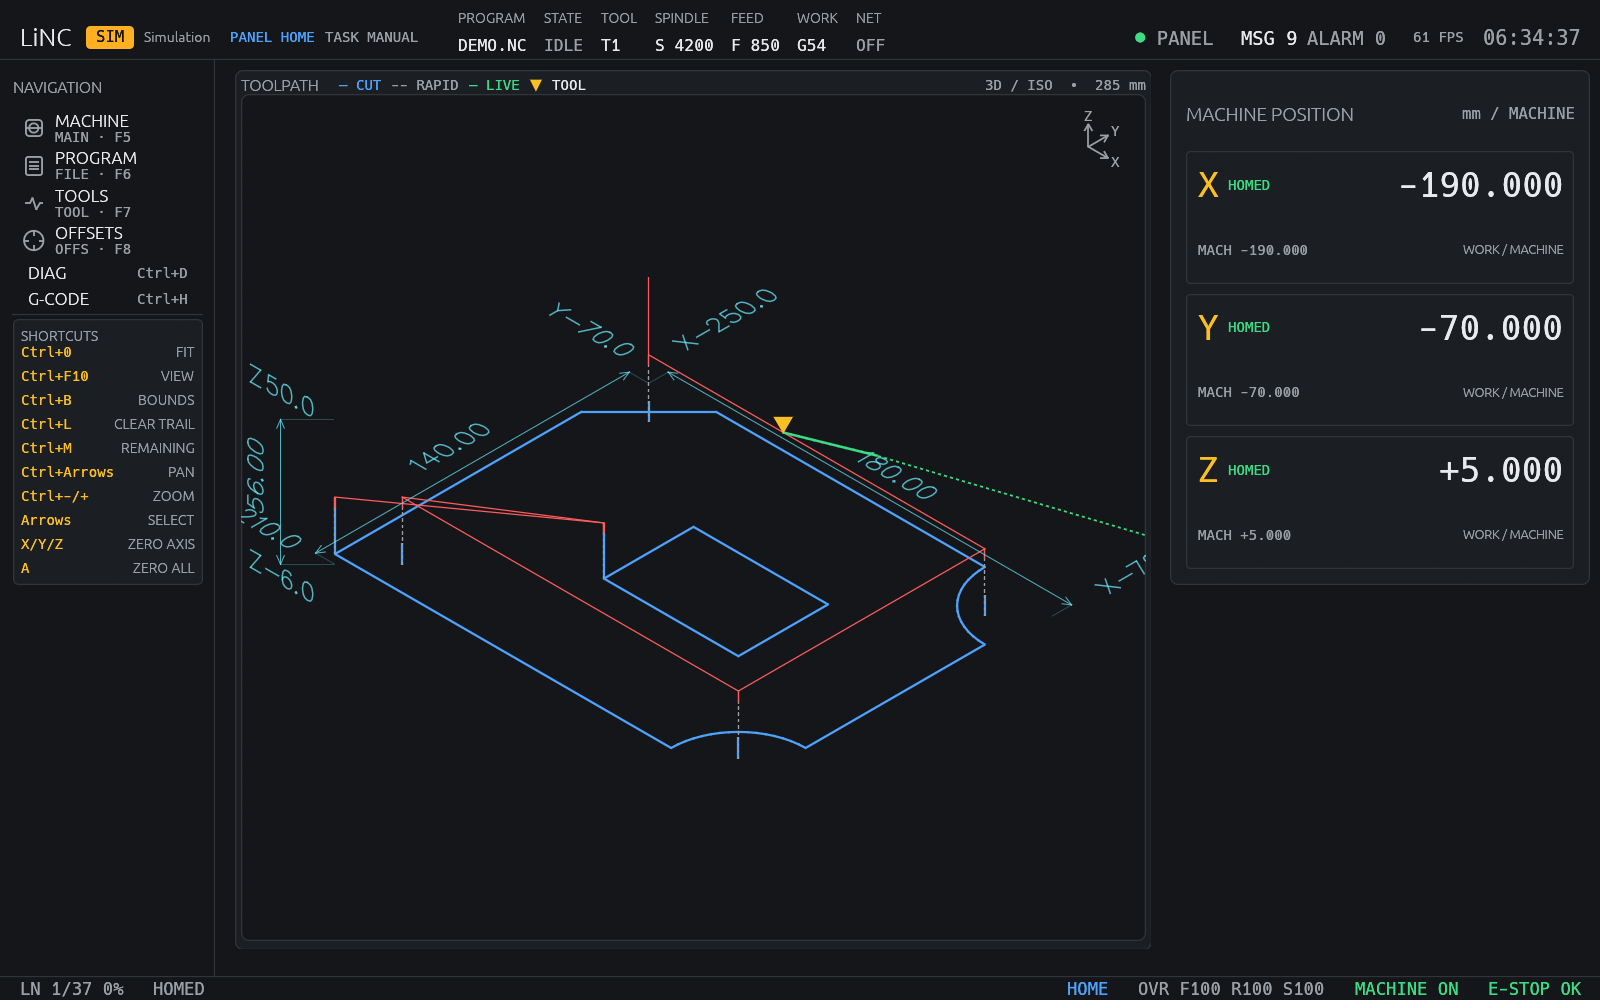
\includegraphics[width=\textwidth]{img/ui/homing.png}
  \caption{The Homing page in HOME mode: machine position with a homing badge per axis, and
           the same toolpath as the Manual page.}
  \label{fig:homing}
\end{figure}

Homing establishes the machine reference. It is required after power-on and after a loss of
reference. Which key homes which axis is the machine's HAL wiring, and the page documents it.

\begin{enumerate}
  \item Turn the selector to \textbf{HOME}. The Homing page opens.
  \item Press \pbtn{RAPID} to home all axes, or the axis key of a single axis.
  \item Each axis row shows a badge: \state{HOMED}, \state{HOMING}, \state{NOT HOMED},
        \state{UNKNOWN} or \state{NOT CONFIGURED}.
  \item The bottom bar changes from \state{NOT HOMED} to \state{HOMED} when every axis is
        home.
\end{enumerate}

The homing order and the search, latch and index settings come from the machine INI and are
shown on the page. With \texttt{NO\_FORCE\_HOMING = 0}, no program and no MDI block runs
before the axes are homed.

\begin{cautionbox}
  Keep a hand near \pbtn{CYCLE STOP} while homing. Check that the table is clear of clamps and
  tools before Z moves.
\end{cautionbox}

\begin{notebox}
  LiNC does not home an axis. The panel's home keys drive the controller's homing input
  directly, which is why homing keeps working when the interface is busy or restarting.
\end{notebox}

\section{PROG.HOME: returning to program zero}

\begin{figure}[H]
  \centering
  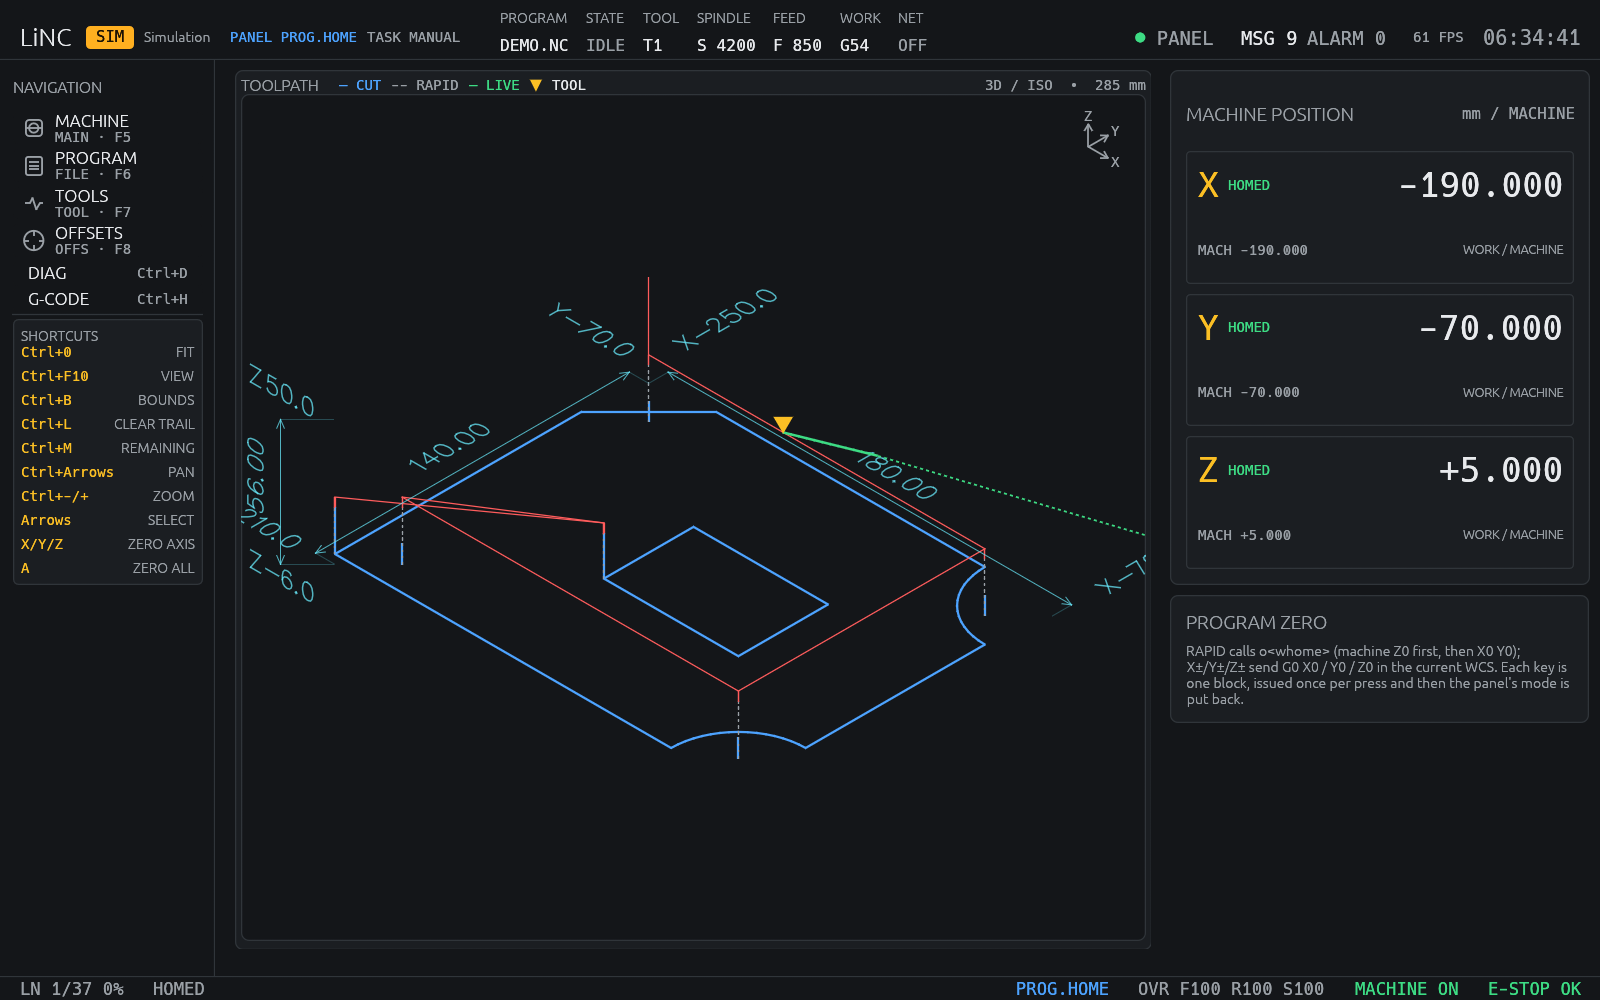
\includegraphics[width=\textwidth]{img/ui/proghome.png}
  \caption{The same page in PROG.HOME mode. The readout is headed \state{PROGRAM ZERO}; the
           panel keys send program-zero blocks.}
  \label{fig:proghome}
\end{figure}

In PROG.HOME the axis keys are not jogs. Each press sends one block, and the interface issues
it:

\begin{center}
\begin{tabular}{ll}
  \toprule
  \textbf{Key} & \textbf{Block} \\
  \midrule
  \pbtn{RAPID} & \texttt{o<whome> call}: machine \texttt{Z0} first, then work \texttt{X0 Y0} \\
  \pbtn{X+} / \pbtn{X-} & \texttt{G0 X0} \\
  \pbtn{Y+} / \pbtn{Y-} & \texttt{G0 Y0} \\
  \pbtn{Z+} / \pbtn{Z-} & \texttt{G0 Z0} \\
  \bottomrule
\end{tabular}
\end{center}

\begin{itemize}
  \item One block per press: a held key does not repeat.
  \item The blocks move to the program zero of the \emph{active} work coordinate system. This
        is not machine home and not \texttt{G53}.
  \item The press is refused, and logged, while the machine is off, an axis is unhomed, the
        interpreter is busy or program protect is on.
  \item The all-axes block lifts Z before it moves X and Y. A single \texttt{G0 X0 Y0 Z0}
        would drag the tool through the part.
\end{itemize}

\section{The Manual page}

\begin{figure}[H]
  \centering
  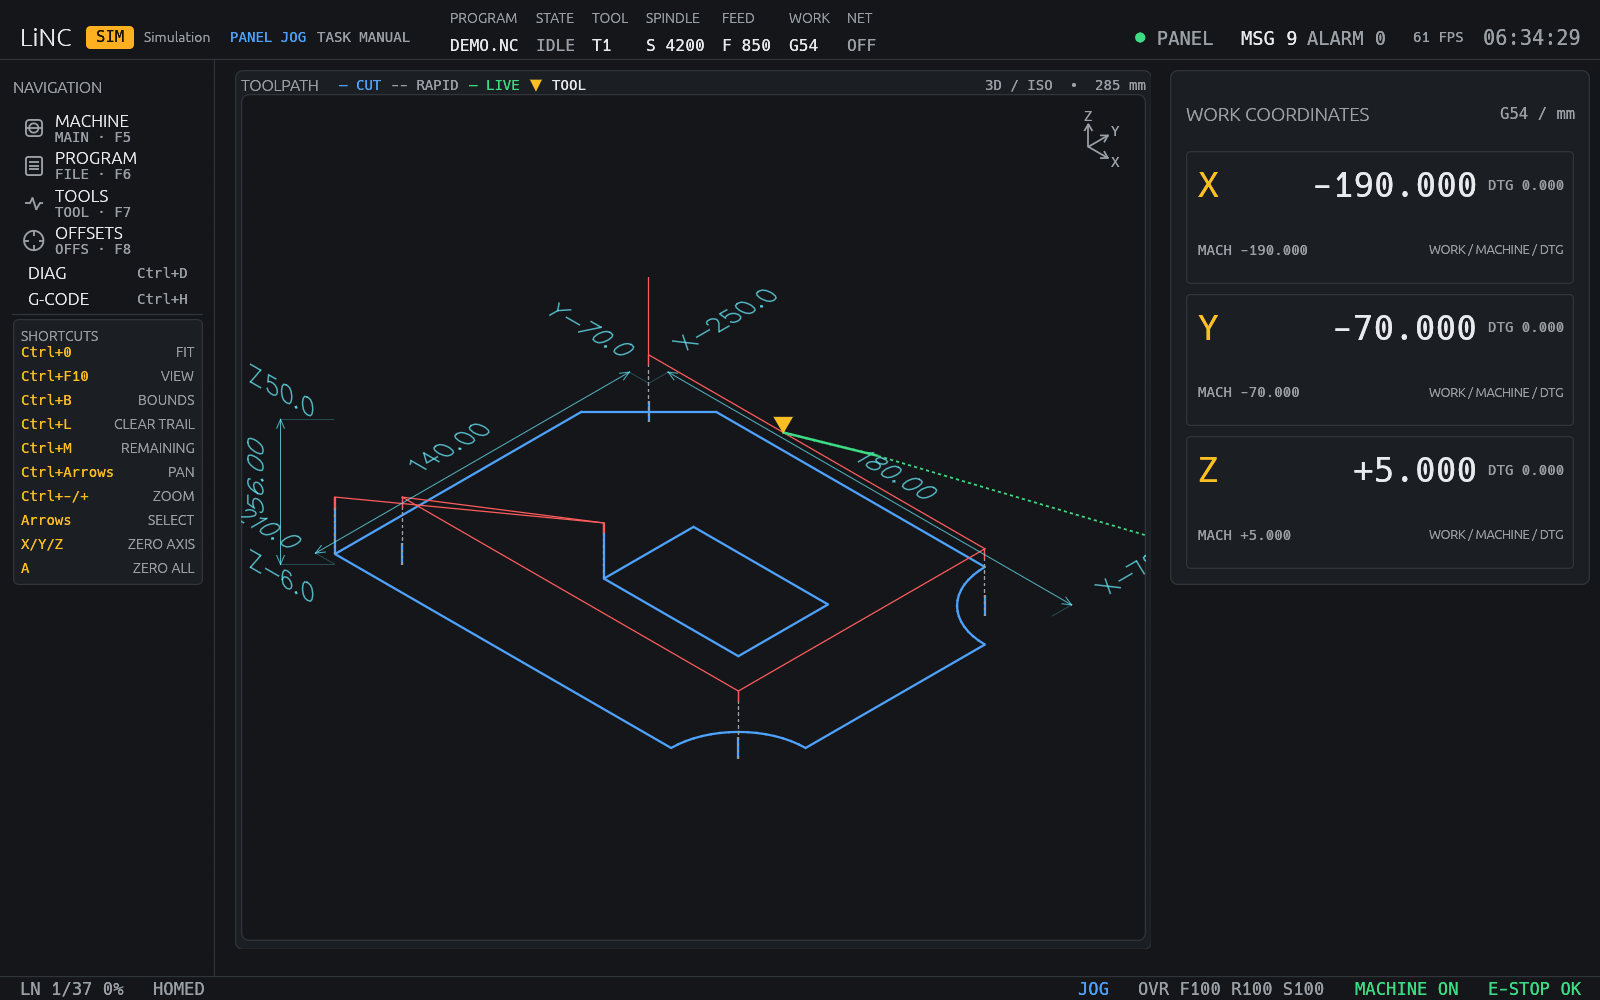
\includegraphics[width=\textwidth]{img/ui/manual.png}
  \caption{The Manual page in JOG mode: toolpath with the loaded program as a muted
           reference, and the work coordinates.}
  \label{fig:manual}
\end{figure}

The Manual page is read-only apart from the increment row and the touch-off keys. It shows:

\begin{itemize}
  \item the toolpath, with the loaded program drawn as a reference and the live trail in its
        own colour;
  \item the work coordinates, the machine coordinates and the distance to go for every axis;
  \item the active axis, highlighted from the panel's axis selection. An unknown selection
        is shown as a dash, never guessed.
\end{itemize}

\begin{tipbox}
  \chordtwo{Ctrl}{0} re-frames the drawing on the tool where it is now. After a long
  jog the trail can drag the view, and a fit brings the part and the tool back together.
\end{tipbox}

\chapter{Running a Program}
\label{ch:running}

A program is loaded in the Files browser, checked on the Program page, and started from the
panel. LiNC never starts a program by itself and never starts one when you load it.

\section{Loading a program}

\begin{itemize}
  \item Press \keycap{F6} for Program, then \keycap{F6} again for Files. On any other page,
        \chordtwo{Ctrl}{O} opens Files directly.
  \item The right-hand pane lists the program directory. It comes from the controller's
        \texttt{PROGRAM\_PREFIX}; there is no second copy of that path in the interface.
  \item The left-hand pane shows removable media. \keycap{Enter} on a file there copies it
        into the program directory.
  \item \keycap{Enter} on a program in the right-hand pane loads it.
\end{itemize}

Loading always does the same four things: it closes Files, switches to Program in the
\sbtn{SPLIT} layout, fits the toolpath and highlights line 1. It does not start anything, and
it does not change the panel's mode.

\begin{cautionbox}
  Only files inside the program directory are loaded. The controller will not accept a path
  outside it, and LiNC does not offer one.
\end{cautionbox}

\shot{img/ui/files.png}{The Files browser: removable media on the left, the program directory on
the right. Every action is a key; there is no button row.}{fig:files}

\section{Checking the program}

\begin{figure}[H]
  \centering
  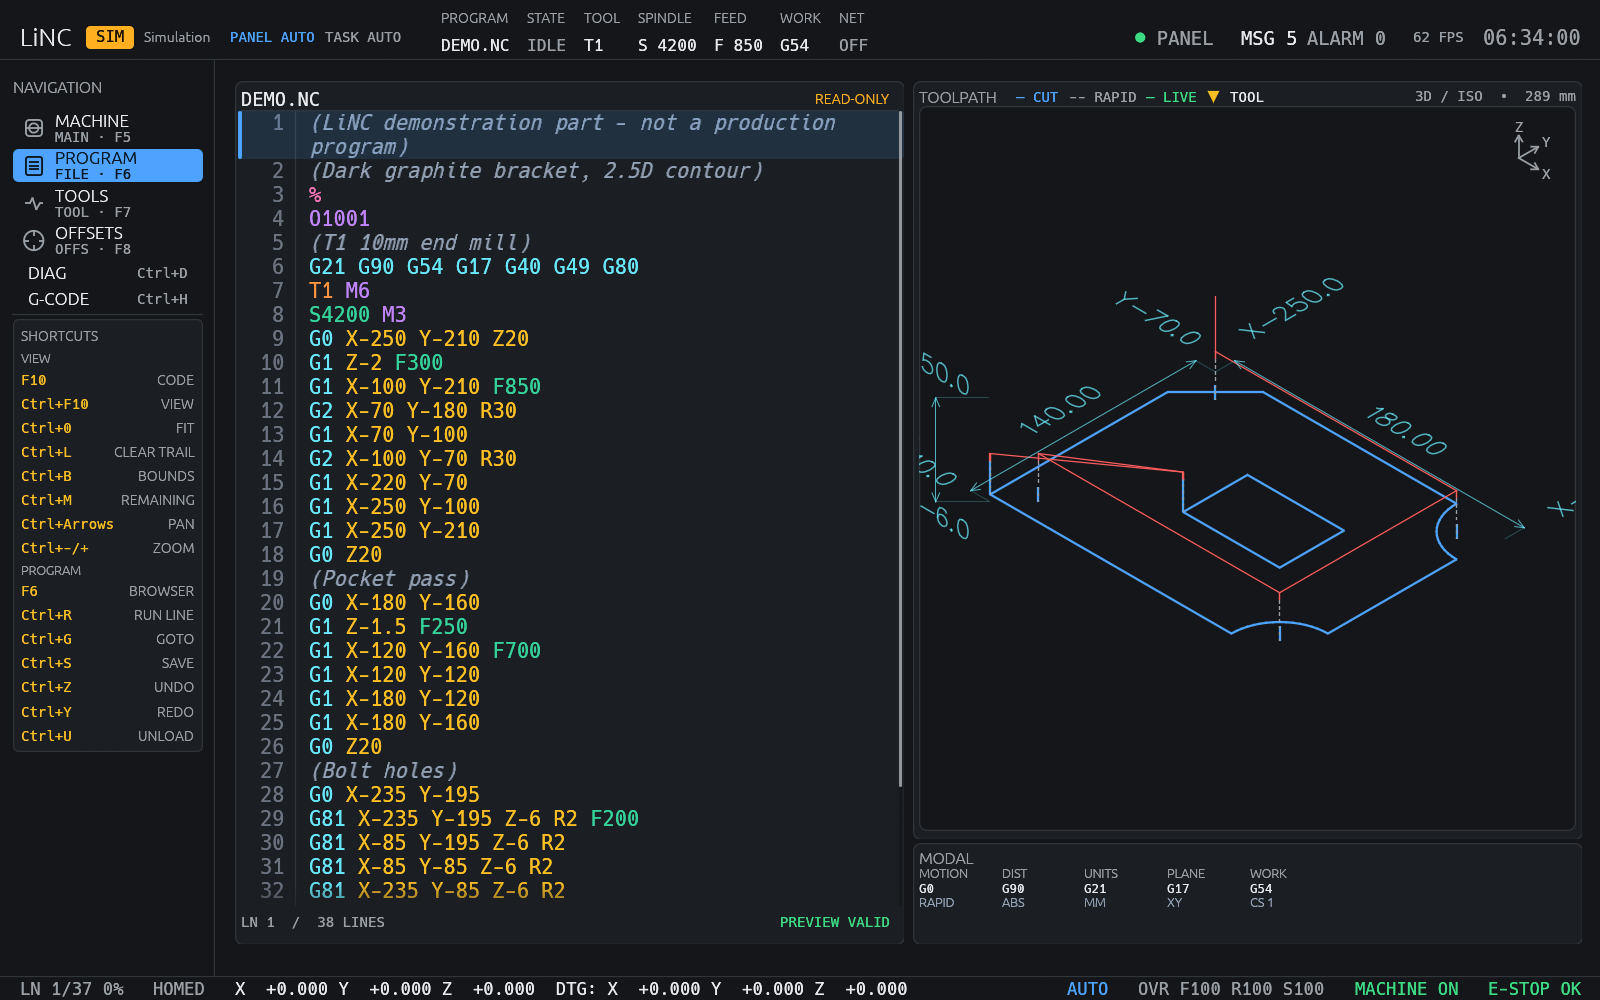
\includegraphics[width=\textwidth]{img/ui/program.png}
  \caption{The Program page in SPLIT: editor or monitor on the left, toolpath on the right,
           modal codes under it.}
  \label{fig:program-page}
\end{figure}

The Program page is the checking surface, and the Machine page is the running surface.

\begin{itemize}
  \item \textbf{The path tells you what the machine will do.} The loaded program is drawn in
        program colours with dotted rapids. Anything outside the machine's travel envelope is
        drawn solid red, split at the exact crossing, so a program that would crash is
        visible before it runs.
  \item \textbf{RED means outside the machine.} It is not a style accent and it is not a
        warning about the toolpath's shape.
  \item \textbf{The preview validates.} A parse error keeps the last valid drawing and marks
        the offending line; it never draws a guess.
  \item \textbf{The modal pane} shows the active units, plane, motion mode, work system and
        compensation, read from the controller as the program runs.
  \item \textbf{The G-code help} answers questions offline: \chordtwo{Ctrl}{H}.
\end{itemize}

The Machine page carries the same toolpath plus the program card: the listing with the
executing line, the modal band, the progress bar and a status word. That word reads
\state{RUNNING}, \state{PAUSED} or \state{STOP}. It is a readout. There is no stop button on
the screen.

\section{Starting the program: cycle start}

The panel's \pbtn{CYCLE START} starts the loaded program. The controller gates it, and the
usual conditions are:

\begin{itemize}
  \item machine power on, no emergency stop,
  \item every axis homed,
  \item the interpreter idle: not running, not waiting for a tool change,
  \item the panel's mode selector in \textbf{AUTO},
  \item panel data current, program protect irrelevant to running but relevant to editing.
\end{itemize}

LiNC does not issue cycle start. It shows the line and the progress, and it shows the
controller's own error in the messages when a start is refused.

\section{Starting at a line: RUN FROM LINE}

\chordtwo{Ctrl}{R} on the Program page starts the loaded program at the selected line.
A line number is the one program-start input the panel cannot supply, so this is the only
program start the interface issues.

\begin{itemize}
  \item It runs only when a program is loaded, the interpreter is idle, the machine is on, no
        emergency stop is latched, every axis is homed, the panel data is current and the
        selector is in AUTO.
  \item A confirmation names the line and its block and states that the lines before it are
        skipped: work and tool offsets, feed, spindle and coolant are not restored, and
        motion starts from the current position.
  \item When a condition blocks it, the reason is shown as a message. The key does not go
        quiet.
\end{itemize}

\section{Finding a line: GO TO LINE}

\chordtwo{Ctrl}{G} asks for a line number and moves the program view there. The editor,
the path highlight and the Machine page's program card follow it. While the program runs the
view normally follows the executing line; a line you chose with \chordtwo{Ctrl}{G} or
the arrow keys is kept until the next run starts.

\section{While the program runs}

\begin{itemize}
  \item The executing line is marked in the listing with a bar and a tinted row, and the view
        scrolls to keep it visible.
  \item The bottom bar shows \state{LN 12/340 34\%}: the executing line, the line count and
        the progress.
  \item The Machine page's toolpath draws the live tool trail in its own colour, separate
        from the program path. \chordtwo{Ctrl}{L} clears the trail without touching
        the program.
  \item \chordtwo{Ctrl}{M} switches to REMAINING: the trail disappears and every block
        already cut is eaten out of the program path, so the card shows only what is left.
  \item Feed hold, single block, block delete, optional stop and cycle stop are panel keys.
        They are wired to the controller, not to LiNC.
\end{itemize}

\begin{notebox}
  The editor is read-only while a program runs. Clicking into the listing selects a line for
  the view; it does not edit the running program, because the controller runs the copy it
  opened, not the buffer.
\end{notebox}

\section{Stopping and resetting}

\begin{itemize}
  \item \pbtn{CYCLE STOP} on the panel stops the program and stops motion.
  \item \keycap{Esc} resets: it aborts the program at the controller and rewinds the
        interpreter. The program stays loaded and can be started again.
  \item A paused program is resumed by cycle start, not by RUN FROM LINE: the controller
        refuses a run-from-line on a paused program rather than resuming it at the wrong
        place.
\end{itemize}

\section{Unloading the program}
\label{sec:unload}

\chordtwo{Ctrl}{U} on the Program page unloads the program and releases the external
network link.

What it does, in order:

\begin{enumerate}
  \item It refuses to run while the program is running (\state{PROGRAM RUNNING — STOP FIRST}),
        with unsaved changes (\state{UNSAVED CHANGES — SAVE OR REVERT FIRST}) or with nothing
        loaded (\state{NO PROGRAM LOADED}).
  \item It sends the controller's program close, then resets the interpreter.
  \item It re-reads the program name from the controller. If the controller still names a
        program, the unload fails loudly with \state{the controller kept the program after
        close} instead of pretending to succeed.
  \item It shows \state{UNLOAD REQUESTED — WATCH NET}. The \state{NET} field returns to
        \state{UP} within a few seconds, once the radio is associated and a default route
        exists.
\end{enumerate}

Unloading also clears the editor and the toolpath on the Program page when the controller
reports that no program is loaded.

\begin{tipbox}
  If the network does not come back, look at the \state{NET} field, not at the WiFi menu.
  \state{?} means the state is unknown; \state{UP} means the link is back. The interface
  writes the interlock's \halpin{net-safe} output and the machine HAL does the rest.
\end{tipbox}

\section{Program changed on disk}

If the file on disk changes while it is open in the buffer, Program shows the banner
\state{PROGRAM CHANGED EXTERNALLY — unsaved buffer preserved. Save will use the current
revision.} The buffer does not reload itself and does not lose your edits. Decide: save over
the new file, or discard and load again.

\chapter{MDI and the G-code Editor}
\label{ch:mdi}

\section{MDI: one block at a time}

MDI is a working area, not a text box. Turn the selector to \textbf{MDI} and the Machine page
opens with the MDI pane in the slot the program card normally fills.

\begin{figure}[H]
  \centering
  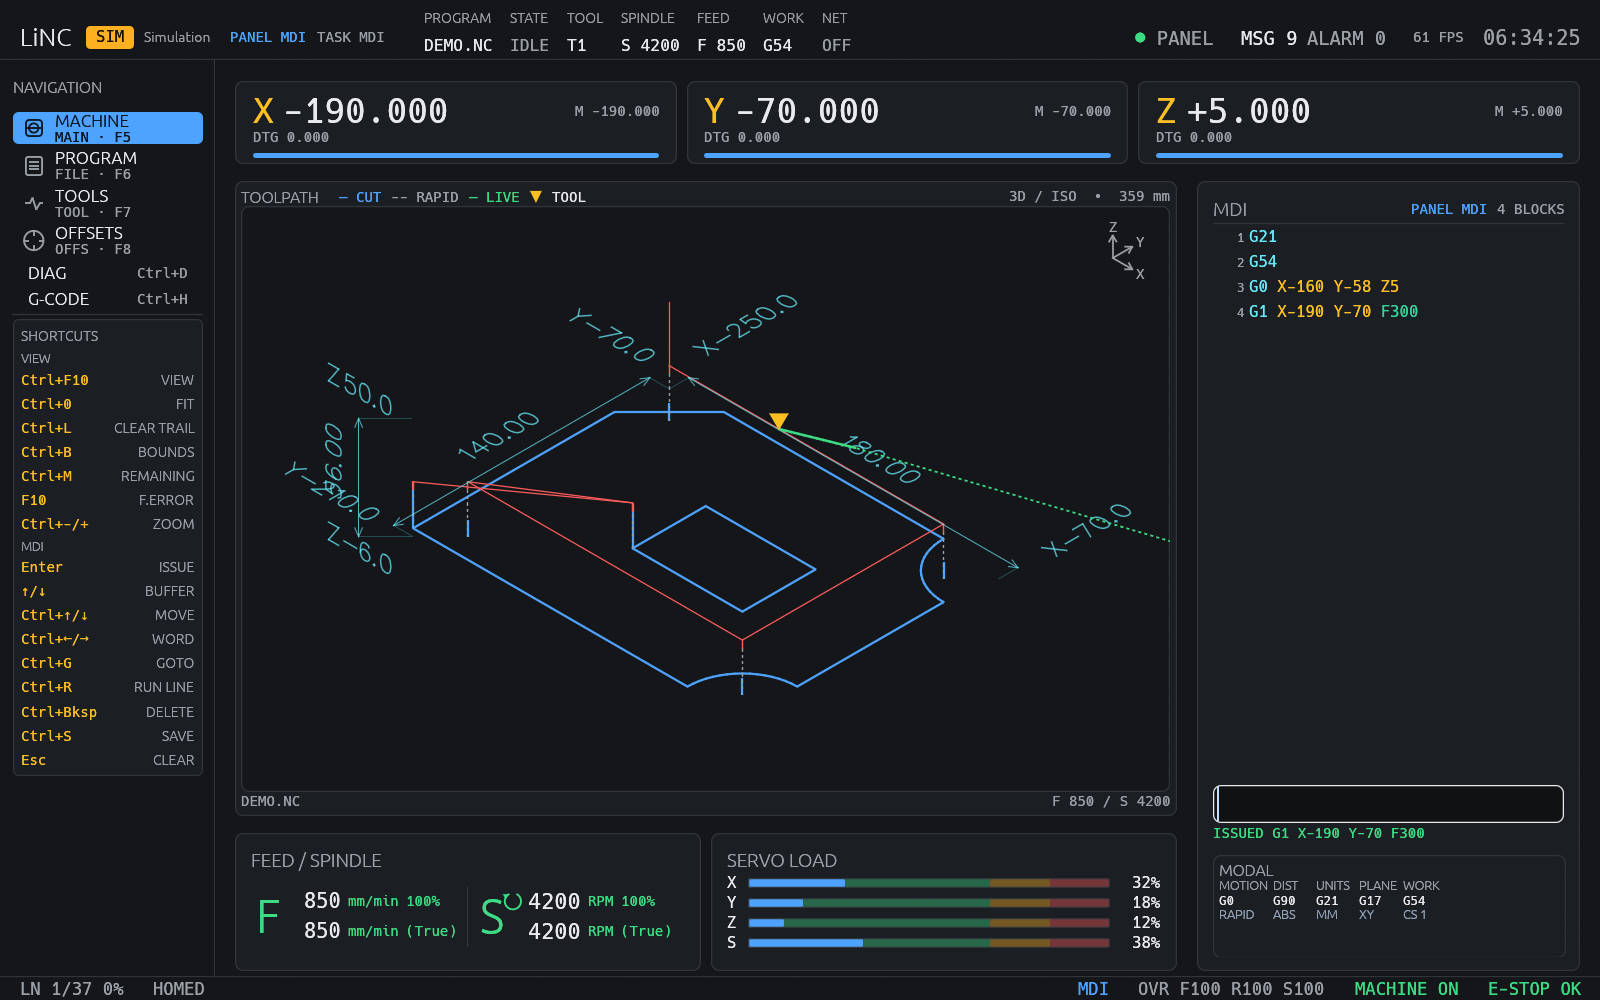
\includegraphics[width=\textwidth]{img/ui/mdi.png}
  \caption{The MDI pane on the Machine page: the blocks already issued, the input line, the
           result strip, the modal band, and the block being typed drawn on the toolpath.}
  \label{fig:mdi}
\end{figure}

The pane, top to bottom:

\begin{itemize}
  \item \textbf{The buffer}: every block issued in this session, in order, with a selection
        band on the row the arrow keys point at.
  \item \textbf{The input}: one syntax-highlighted line. It holds the keyboard by default, so
        a block can be typed as soon as the pane appears.
  \item \textbf{The result strip}: the last issue result, or the validation error that stopped
        it.
  \item \textbf{The modal band}: the same active codes the AUTO program card shows.
\end{itemize}

\subsection*{Keys}

\begin{longtable}{L{4.4cm}L{8.4cm}}
  \toprule
  \textbf{Keys} & \textbf{Action} \\
  \midrule
  \endhead
  \keycap{Enter} & Issue the block. It is committed to the buffer on success. \\
  \keycap{\textuparrow} / \keycap{\textdownarrow} & Move through the buffer and recall that line into the input for
        editing. Recall edits in place: the line stays in the listing while it is being
        edited. \\
  \chordtwo{Ctrl}{\textuparrow} / \chordtwo{Ctrl}{\textdownarrow} & Move the selected buffer line up or down. \\
  \chordtwo{Ctrl}{\textleftarrow} / \chordtwo{Ctrl}{\textrightarrow} & Move by word in the input. \\
  \chordtwo{Ctrl}{G} & Go to a buffer line. \\
  \chordtwo{Ctrl}{R} & Issue the selected buffer line directly, with no confirmation. \\
  \chordtwo{Ctrl}{Backspace} & Delete the selected buffer line; with no line,
        clear the input. \\
  \chordtwo{Ctrl}{S} & Save the buffer as a program file. \\
  \keycap{Esc} & Clear the uncommitted input. An already issued block is not cancelled. \\
  \bottomrule
\end{longtable}

\subsection*{What the pane refuses}

\begin{itemize}
  \item A block issues only when the machine is on, every axis is homed, the interpreter is
        idle, no program is loaded and the selector is in MDI.
  \item A syntax error issues nothing and marks the input.
  \item The controller is switched to MDI for the block and put back afterwards. No physical
        cycle start is involved.
  \item The preview of the block is refused, not clipped, when it would leave the machine's
        travel envelope.
\end{itemize}

\subsection*{The preview}

The block you are typing is drawn on the Machine page's toolpath, over the loaded program, in
the MDI preview colour: dashed for a rapid, solid for a cut. Its move starts at the machine's
current position. This is what makes MDI safe to use for a quick approach: the move is on the
screen before it is sent.

The preview understands \texttt{G91}: a relative move is drawn where it will go, not where
its words would put it in absolute mode.

\begin{notebox}
  An empty, unparsable or over-long block draws nothing extra. The strip says why, and the
  pane will refuse it.
\end{notebox}

\subsection*{Saving the buffer}

\chordtwo{Ctrl}{S} writes the buffer to a new \texttt{.ngc} file in the program
directory. The dialog asks for a name and offers an \sbtn{add pre/postamble} checkbox. Ticked,
the file gets the profile's preamble above the buffer and its postamble below.

The buffer is kept across page changes and restarts. It is an interface working list, not a
machine log.

\section{The G-code editor}

Turn the selector to \textbf{EDIT}. The Program page opens in the \sbtn{CODE} layout with the
editor focused and editable. The panel's selector is the authority: outside EDIT the buffer
is read-only, whatever page is in front.

\begin{itemize}
  \item \textbf{Layout.} \keycap{F10} toggles SPLIT and CODE. SPLIT is for reading a program
        beside its path; CODE is for editing, with a narrow path thumbnail.
  \item \textbf{Highlighting.} G-codes, M-codes, axis letters, numbers, feed and speed, tool
        words, parameters and comments each have their own colour. Comments are italic.
  \item \textbf{Line numbers, current line and the dirty marker.} An edited buffer marks
        itself in the header and accents \sbtn{SAVE} until it is saved.
  \item \textbf{The preview} updates from a debounced parse. Invalid G-code keeps the last
        valid drawing and marks the failing line. The preview never moves the machine.
\end{itemize}

\begin{longtable}{L{4.7cm}L{8.1cm}}
  \toprule
  \textbf{Keys} & \textbf{Action} \\
  \midrule
  \endhead
  \chordtwo{Ctrl}{S} & Save. \\
  \chordtwo{Ctrl}{Z} / \chordtwo{Ctrl}{Y} & Undo / redo. \\
  \chordtwo{Ctrl}{A} / \keycap{C} / \keycap{X} / \keycap{V} & Select all, copy, cut,
        paste. \\
  \chordtwo{Ctrl}{G} & Go to a line. \\
  \chordtwo{Ctrl}{D} & Duplicate the current line. \\
  \chordtwo{Ctrl}{K} & Delete the current line. \\
  \chordtwo{Ctrl}{\textuparrow} / \chordtwo{Ctrl}{\textdownarrow} & Move the current line up or down. \\
  \chordtwo{Ctrl}{\textleftarrow} / \chordtwo{Ctrl}{\textrightarrow} & Move by word. \\
  \keycap{Home} / \keycap{End} & Start / end of the line. \\
  \keycap{PgUp} / \keycap{PgDn} & A screenful up or down, or to the start and end of a
        program shorter than one screen. \\
  \bottomrule
\end{longtable}

The editor applies the same spacing rule as MDI: a word typed against anything that is not a
space gets one space in front of it, so \texttt{G1X10} arrives as \texttt{G1 X10} and
\texttt{X10G0} as \texttt{X10 G0}. Nothing is inserted inside a comment or an expression, and
nothing at all when text is pasted.

\subsection*{Saving}

Saving is explicit. There is no autosave. A save is allowed only when:

\begin{itemize}
  \item the panel is in \textbf{EDIT},
  \item the interpreter is idle,
  \item program protect is off.
\end{itemize}

A buffer that has no file yet asks for a name. The dialog shows the program directory, appends
the configured G-code extension when the name has none, refuses a name that already exists, and
keeps the buffer on that path for later saves.

After writing, the controller is given the saved file again, so AUTO runs the text you saved,
not the copy the interpreter opened before the edit.

\begin{cautionbox}
  Protect and a running program both refuse a save. The unsaved-changes dialog greys
  \sbtn{SAVE} and names the blocking condition instead of letting the key do nothing.
\end{cautionbox}

\subsection*{Unsaved changes}

The buffer is protected against being lost by accident:

\begin{itemize}
  \item Leaving Program, opening another file or quitting with a dirty buffer raises a
        confirmation.
  \item \sbtn{DISCARD} really drops the buffer: it is reloaded from the loaded program, or
        emptied when nothing is loaded, before the destination is entered.
  \item Leaving EDIT with a dirty buffer warns that AUTO can only start the loaded file, and
        offers \sbtn{DISCARD BUFFER} or \sbtn{KEEP}.
  \item Switching protect on keeps the buffer and its dirty marker, read-only, until the
        switch is off.
\end{itemize}

While a program runs the editor is read-only and scrolls to the executing line. The controller
runs its own copy; editing the buffer mid-run was never going to change the cut.

\chapter{Tools, Offsets and Tool Changes}
\label{ch:tools}

\section{The tool table}

\begin{figure}[H]
  \centering
  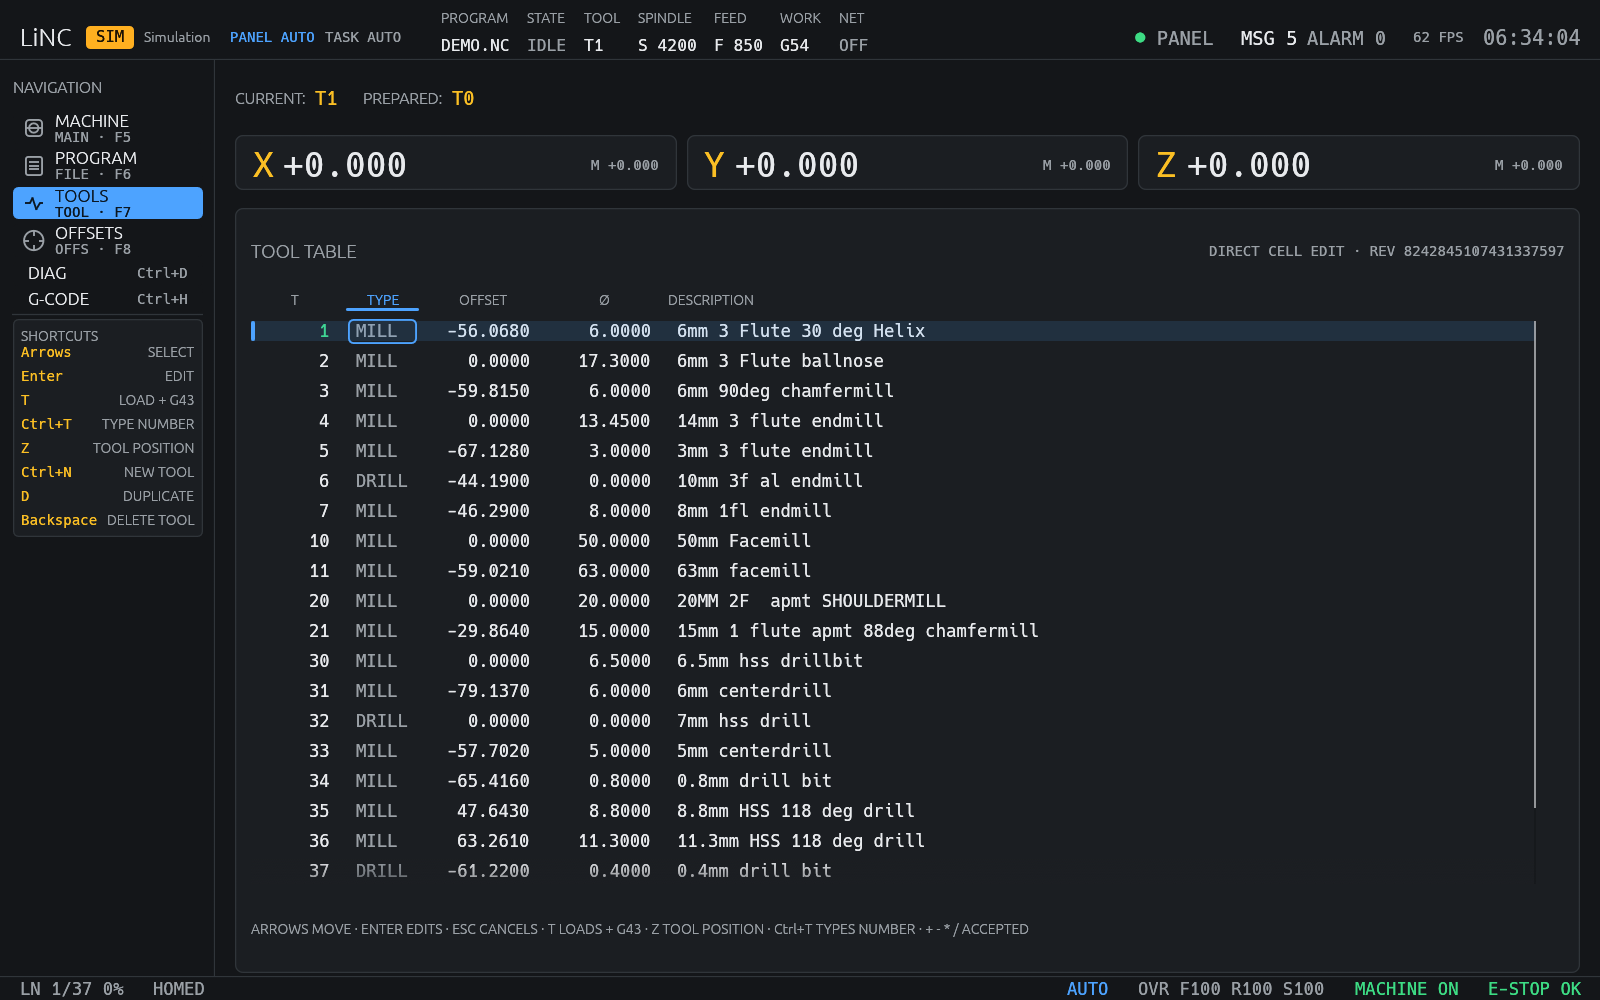
\includegraphics[width=\textwidth]{img/ui/tools.png}
  \caption{The Tools page. The table is the page: there is no separate change pane and no
           changer pane.}
  \label{fig:tools}
\end{figure}

The Tools page reads and writes the controller's standard tool table, the file named by
\texttt{[EMCIO] TOOL\_TABLE} in the machine INI. The columns come from the table's own
\texttt{TOOL\_TABLE\_COLUMNS}, so the page shows the schema the machine actually has.

Above the table, the current and prepared tools are named: \sbtn{CURRENT: T3},
\sbtn{PREPARED: T7}. A pocket column appears only on a machine with an automatic changer; a
manual-change machine hides it.

\begin{longtable}{L{3.2cm}L{9.6cm}}
  \toprule
  \textbf{Keys} & \textbf{Action} \\
  \midrule
  \endhead
  Arrows & Move through the table and its rows. The table takes the keyboard when the page
        opens. \\
  \keycap{Enter} & Edit the selected cell. The whole value is selected. \keycap{Enter} writes
        it; \keycap{Esc} restores the previous value. \\
  \keycap{T} & Load the selected row's tool: \texttt{Tn M6} and \texttt{G43 Hn} in one
        command, so length compensation is in effect when the change completes. \\
  \chordtwo{Ctrl}{T} & Type a tool number instead of cursoring to its row. \texttt{0}
        unloads the spindle. \\
  \keycap{Z} & Open the tool position dialog for the tool in the spindle. \\
  \chordtwo{Ctrl}{N} & Add a row with the next free tool number. \\
  \keycap{D} & Duplicate the selected row under the next free number. \\
  \keycap{Backspace} & Delete the selected row after a confirmation. \\
  \keycap{S} & Run one Loobric sync, when the machine has a Loobric server. \\
  \bottomrule
\end{longtable}

\begin{itemize}
  \item Writing a cell reloads the table into the controller and re-applies \texttt{G43} when
        the edited row is the tool in the spindle. The interface waits until the controller
        publishes the new row, so compensation cannot run against the table it is replacing.
  \item The probe tool and the tool in the spindle cannot be deleted, and the probe tool
        number is skipped when a new row is created.
  \item The `Z' column and the length field are one offset under two names: either cell writes
        both.
  \item An edited cell turns red while it holds an uncommitted value.
\end{itemize}

\section{The tool position dialog}

\keycap{Z} opens one line: \sbtn{SET <axis> POSITION}, the entry, and the offset the confirm
would write. It asks where the tool is now, seeded with the work coordinate the controller
reports, and writes the tool offset so the work coordinate reads the entered value.

\begin{itemize}
  \item \keycap{X}, \keycap{Y} and \keycap{Z} choose which coordinate is being entered.
  \item A \keycap{Z} entry updates the tool's length. \keycap{X} and \keycap{Y} update the
        geometry offsets the same way.
  \item The entry accepts arithmetic: \texttt{-12.5} and \texttt{10+2.5} both work.
  \item A refused write (machine off, running, protect, panel offline) keeps the dialog open
        and names the reason.
\end{itemize}

\section{Tool numbers without cursoring}

\chordtwo{Ctrl}{T} opens a one-line tool-number dialog, prefilled with the tool in the
spindle and fully selected, so \keycap{Enter} alone re-loads that tool.

Only a number the table carries, or \texttt{0}, is accepted. A refusal names the problem
(\texttt{T7 is not in the tool table}, an empty entry, a non-numeric one) and keeps the dialog
open.

\section{Manual tool changes}

On a machine with a manual changer, \texttt{M6} pauses for the change and a prompt appears --
on every page, not only on Tools:

\begin{description}[font=\normalfont\sffamily\bfseries, leftmargin=3.4cm, style=nextline]
  \item[\sbtn{INSTALL}] The tool to put in the spindle.
  \item[\sbtn{REMOVE}] The tool to take out, with its description.
  \item[\sbtn{CONFIRM}] The only action. It confirms that the tool is in.
\end{description}

The prompt follows the controller's request and cannot be dismissed. Confirming is a
handshake, not motion: it is allowed while the program is running or paused, and it does not
need cycle start. It raises the declared \halpin{linc.tool-change-confirm} output and holds it
until the controller drops its own request, so a short pulse cannot be missed.

Until it is confirmed, the bottom bar shows \state{TC T7 PENDING}.

\begin{safetybox}
  Check that the tool is seated and clamped before confirming. The controller continues the
  program immediately after the confirmation.
\end{safetybox}

\section{The tool in the spindle survives a restart}

The controller starts a fresh session with an empty spindle, even when the previous session
left a tool in it. LiNC remembers the tool number in a state file beside its preferences and
restores it with \texttt{M61 Qn} and \texttt{G43 Hn} once the machine is on, homed, idle and
unprotected, and the tool is in the table.

A controller that already reports a tool wins; the remembered number is only used when the
controller reports an empty spindle.

\section{Loobric tool-table sync (optional)}

A machine with a Loobric server can keep its tool table in step with it. When the profile has
a \texttt{[loobric]} section, the Tools page shows the sync state in its header and accepts
\keycap{S} for a manual sync.

\begin{center}
\begin{tabular}{ll}
  \toprule
  \textbf{State} & \textbf{Meaning} \\
  \midrule
  \state{syncing...} & A sync is running. \\
  \state{tool write waiting for idle} & A local tool change is waiting to be sent. \\
  \state{server changes waiting for idle} & The server has changes to bring in. \\
  \state{not synced yet} & Nothing has been exchanged in this session. \\
  \bottomrule
\end{tabular}
\end{center}

Syncs wait for an idle machine. A tool write made just before starting a program is sent when
the machine is idle again, not in the middle of a cut. \keycap{S} refuses with
\state{Loobric sync waits for idle} while a program runs, which is the same rule the automatic
sync keeps.

\section{Work offsets}

\begin{figure}[H]
  \centering
  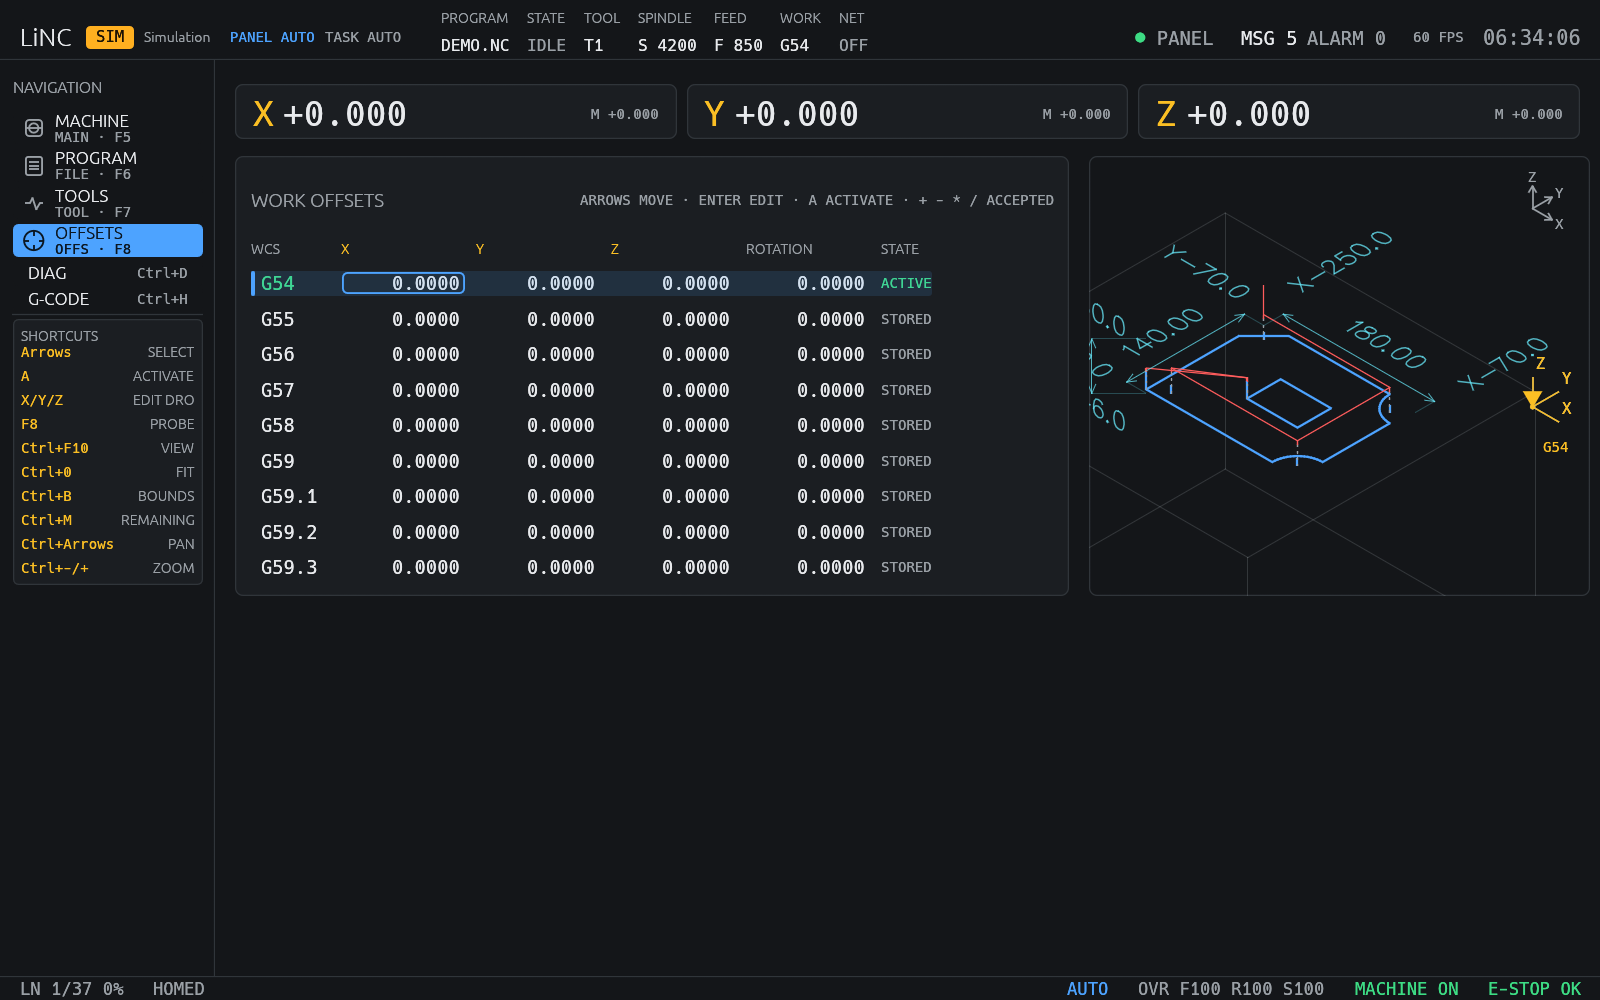
\includegraphics[width=\textwidth]{img/ui/offsets.png}
  \caption{The Offsets page: the DRO row, the nine work coordinate systems with rotation, and
           the preview drawn in machine space.}
  \label{fig:offsets}
\end{figure}

The Offsets page holds the nine work coordinate systems the controller numbers,
\texttt{G54} to \texttt{G59.3}, each with a rotation column, plus the tool offsets.

\begin{itemize}
  \item \textbf{The DRO row} shows the active system's work coordinates large, with the machine
        coordinate small underneath. A work value is edited in place and accepts arithmetic;
        committing writes the position with \texttt{G10 L20}, so the DRO reads the value you
        entered and the offset moves to match.
  \item \textbf{\keycap{A}} makes the highlighted row the active system without leaving the
        page. The controller selects it with an MDI block, and the interface verifies the
        active index it reports afterwards.
  \item \textbf{\keycap{X}}, \keycap{Y} and \keycap{Z} open the DRO for that axis.
  \item \textbf{\keycap{F8}} moves on to the probe tabs; \keycap{Esc} comes back here.
  \item \textbf{The preview} is drawn in machine space in the work system the program selects,
        so the part sits where it will be cut. The view keys work as everywhere else
        (\chordtwo{Ctrl}{F10}, \chordtwo{Ctrl}{0}, \chordtwo{Ctrl}{B},
        \chordtwo{Ctrl}{M}, \keycap{Ctrl}+arrows, \mbox{\keycap{Ctrl}+\texttt{+}/\texttt{-}}).
\end{itemize}

G92 is deliberately not exposed here. It is a transient shift that silently moves every work
system, and a field for it invited a machine state that neither the DRO nor a program could
explain.

\begin{cautionbox}
  A work offset moves the program, not the machine. The preview shows the effect before you run
  anything: check where the part sits after an edit, especially after a rotation.
\end{cautionbox}

\chapter{Touch Probing}
\label{ch:probing}

The probe page turns the touch probe into a guided measuring tool: choose a category, pick an
illustrated operation, set the parameters, run it, read the result. The probing math is not
reimplemented -- the Probe Basic G-code routines ship with LiNC and run as they are.

Probing is available on a mill profile with a probe configured. On the Offsets page, \keycap{F8}
moves into the probe tabs.

\shot{img/ui/probe.png}{The probe page: editable DRO and parameters on the left, the routine
matrix in the centre, the probe and results on the right.}{fig:probe}

\section{The tabs}

\begin{center}
\begin{tabular}{ll}
  \toprule
  \textbf{Tab} & \textbf{What it measures} \\
  \midrule
  \state{OUTSIDE CORNERS} & X/Y faces and corners from outside the part \\
  \state{INSIDE CORNERS} & Faces and corners from inside a pocket \\
  \state{BOSS AND POCKET} & Round and rectangular bosses and pockets: width, centre, diameter \\
  \state{RIDGE AND VALLEY} & Ridges, valleys and their centres \\
  \state{EDGE ANGLE} & The angle of an edge, and applying it as a work rotation \\
  \state{CALIBRATE} & Probe calibration: round and square boss and pocket, offsets, reset \\
  \state{PROBE HELP} & The Probe Basic help text, page by page \\
  \bottomrule
\end{tabular}
\end{center}

\keycap{F8} moves to the next tab and \keycap{PgUp}/\keycap{PgDn} cycle them; \keycap{Esc}
returns to Offsets. The tabs are indicators, not buttons, and take no keyboard focus.

\section{The page}

\begin{itemize}
  \item \textbf{Top left:} an editable work-coordinate DRO. \keycap{X}, \keycap{Y} and
        \keycap{Z} open that axis, \keycap{Enter} writes the work position with
        \texttt{G10 L20}, \keycap{Esc} cancels. Work offsets themselves stay on the Offsets
        page; the header names the active system.
  \item \textbf{Below it:} the parameter card, with the probe tool, the fast, slow and
        traverse feed rates, the maximum X/Y and Z distance, the clearances, the extra depth,
        the edge width and the diameter hints. Arithmetic is accepted, as in the offset cells.
  \item \textbf{Centre:} the illustrated routines of the selected tab. \keycap{1} to
        \keycap{9} highlight a routine. \keycap{Enter} runs it.
  \item \textbf{Right:} the probe symbol and the results of the last run.
\end{itemize}

No routine is selected when the page opens or a tab changes. A number key is the only way to
select one; \keycap{Enter} before that reports that a routine must be selected.

\begin{tipbox}
  The keys that matter are listed in the pane under the navigation column: \state{PROBE KEYS}
  and \state{RESULT KEYS}. After an hour away from the machine, that pane is faster than this
  chapter.
\end{tipbox}

\section{Position and direct: the W key}

\keycap{W} switches what a run does with its result, and the screen says which mode is active:

\begin{description}[font=\normalfont\sffamily\bfseries, leftmargin=3.4cm, style=nextline]
  \item[\state{POSITION}] The default. The routine measures and records. Nothing is written to
        a work offset; \keycap{A} applies the last result when you decide to.
  \item[\state{DIRECT WCO}] The routine writes the active work offset itself, in the issued
        block. It needs a valid active offset, and it is refused when protect is on.
\end{description}

\section{Running a routine}

\keycap{Enter} builds the selected \texttt{o<probe\_...> call} and its argument values and
issues it immediately. The controller is switched to MDI for the block and the previous task
mode is restored when the interpreter returns idle. No physical cycle start is involved.

A run requires:

\begin{itemize}
  \item machine power on and every axis homed,
  \item the probe tool in the spindle,
  \item an idle interpreter and no active program,
  \item valid parameters.
\end{itemize}

A validation error issues nothing and marks the failing condition.

\begin{cautionbox}
  A probe cycle moves the machine. Check the clearance values and the probe tool before
  \keycap{Enter}. The fast feed rate is the approach; the slow feed rate is the contact.
\end{cautionbox}

\section{The results}

Results come from the subroutine outputs and are shown as named slots: \state{X WIDTH},
\state{X CENTRE}, \state{Y WIDTH}, \state{Y CENTRE}, \state{X- FACE}, \state{X+ FACE},
\state{Y- FACE}, \state{Y+ FACE}, \state{Z SURFACE}, \state{AVG DIAM} and
\state{EDGE DELTA}.

\begin{longtable}{L{4.7cm}L{8.1cm}}
  \toprule
  \textbf{Keys} & \textbf{Action} \\
  \midrule
  \endhead
  \keycap{A} & Apply the last result to the active work offset. Protect must be off. \\
  \keycap{U} & Update the probe parameters from the last result. \\
  \chordtwo{Ctrl}{R} & Reset all probe data. \\
  \chordtwo{Ctrl}{X} / \chordtwo{Ctrl}{Y} & Reset the X or the Y data. \\
  \bottomrule
\end{longtable}

The results panel carries no buttons: those keys are the whole surface.

\section{Edge angle and work rotation}

On \state{EDGE ANGLE}, \keycap{R} applies the measured angle as the active work coordinate
rotation. Check the Offsets page afterwards: the rotation appears there, and the preview shows
the part rotated around its zero.

\section{Calibration}

The \state{CALIBRATE} tab measures the probe against a known feature and stores the calibration
offset. Its fields -- known width or diameter, calibration axis and the calibration offset
itself -- live on the same panel.

\begin{itemize}
  \item \keycap{1} to \keycap{4} highlight a calibration routine; \keycap{Enter} runs it.
  \item \keycap{V} switches the calibration between the averaged XY result and the single X or
        Y result.
  \item \chordtwo{Ctrl}{P} reaches the calibration dimensions.
  \item \chordtwo{Ctrl}{R} resets the calibration through the Probe Basic reset routine.
\end{itemize}

\section{When the probe is hit}

If the probe input rises during a move that is not a probe, the controller aborts the move and
reports an operator error. LiNC latches it: a red banner carries the controller's text on every
page, motion and MDI are blocked, and the machine is switched off unless it was paused with
nothing moving.

\keycap{Esc} clears the latched trip from any page. Re-powering afterwards needs a fresh
\pbtn{ON} at the panel. The full behaviour is in chapter~\ref{ch:power}.

\begin{notebox}
  The probe input is also shown in the bottom bar, but only while the probe tool is in the
  spindle: \state{PROBE READY} or \state{PROBE TRIPPED}. There is no probe field for a cutter in
  the spindle, because there is no probe to read.
\end{notebox}

\chapter{Diagnostics and Troubleshooting}
\label{ch:diagnostics}

\chordtwo{Ctrl}{D} opens Diagnostics. The page is read-only: nothing here jogs, cycles,
resets or acknowledges. It exists to answer three questions -- is the controller healthy, what
did it say, and what is the machine actually doing -- and to let you read the answer without a
terminal.

\shot{img/ui/diagnostics.png}{Diagnostics, OVERVIEW tab: four health cards, the panel link
strip, and the active alarms and messages.}{fig:diagnostics}

\section{OVERVIEW}

\begin{center}
\begin{tabular}{L{3.0cm}L{5.0cm}L{5.0cm}}
  \toprule
  \textbf{Card} & \textbf{Values} & \textbf{Detail line} \\
  \midrule
  \state{CONTROL} & \state{HEALTHY} or \state{E-STOP} & task mode / interpreter state \\
  \state{PANEL LINK} & \state{ONLINE} or \state{OFFLINE} & transport, port, CRC errors,
        timeouts \\
  \state{NML / COMMAND} & \state{CONNECTED} or \state{LOST} & status age, echo serial \\
  \state{MOTION} & \state{NOMINAL} or \state{ELEVATED} & largest following error in µm,
        largest servo load in percent \\
  \bottomrule
\end{tabular}
\end{center}

\state{ELEVATED} means a following error above 50\,µm. It is a warning threshold, not a fault:
look at the axes and the load, and at the machine's own limits.

Below the cards, the \textbf{panel link strip} shows the transport, the last receive time and
its age. A transport that keeps no byte counters says so instead of showing invented ones.

\section{LOGS}

The event history, newest entries first, with the time, severity, source, code and message.
The severity and source filters are toggles; the status line reports which are on, and shows
\state{ALL} for a group with nothing selected.

\begin{longtable}{L{4.7cm}L{8.1cm}}
  \toprule
  \textbf{Keys} & \textbf{Action} \\
  \midrule
  \endhead
  \keycap{/} & Focus the search line. Matches message, code and source. \\
  \keycap{Enter} & Leave the search line and take the list. \\
  \keycap{Esc} & Leave the list and return to the search line. \\
  \keycap{I} \keycap{W} \keycap{E} \keycap{C} & Toggle INFO, WARN, ERROR and CRIT severity
        filters. \\
  \keycap{P} \keycap{G} \keycap{B} \keycap{T} \keycap{H} & Toggle PANEL, PROGRAM, PROBE, TOOL
        and HAL sources. \\
  \keycap{N} \keycap{M} \keycap{O} \keycap{U} \keycap{Y} & Toggle NML, MOTION, I/O, UI and
        SYSTEM sources. \\
  \keycap{A} & Clear all filters. \\
  \keycap{PgUp} / \keycap{PgDn} & Scroll a list that overflows, otherwise change tab. \\
  \bottomrule
\end{longtable}

\begin{notebox}
  The letter toggles act only while the list holds the keyboard. In the search line the same
  letters are text -- which is how you search for a word containing an \texttt{e}.
\end{notebox}

\section{HAL / NML}

The \textbf{NML / COMMAND} status line at the top, then the HAL browser: pins grouped by
component, each with its type, direction, value and signal, and a separate signal list.

\begin{itemize}
  \item \keycap{/} focuses the search, \keycap{Enter} takes the list, \keycap{Left} and
        \keycap{Right} switch between pins and signals, and \keycap{Esc} returns to the search.
  \item \keycap{F} and \keycap{S} refresh faster or slower. The header shows the age of the
        rows it drew.
  \item The browser shells out to \halpin{halcmd show pin} and \halpin{halcmd show sig} on a
        background thread. Without a running controller or without \halpin{halcmd} it says so
        and shows nothing; it never fills the tree in from the machine snapshot.
  \item Nothing on this tab writes to HAL.
\end{itemize}

\begin{tipbox}
  The HAL browser is the fastest way to see whether a panel key or a limit switch actually
  reaches the controller: search for the pin, press the key, watch the value change.
\end{tipbox}

\section{Messages}

\keycap{M} opens the full-screen message list from any page. It carries the same rows as the
LOGS tab, without filters, and closes with \keycap{Enter} or \keycap{Esc}.

\section{Where the session log goes}

The interface writes its own log (errors, warnings, the start-up line naming the profile and
the loaded program) to standard error. The machine's launcher redirects it into the profile's
log directory, for example \texttt{logs/linc.log}. Read it when the interface closed with a
message but the screen is gone.

\section{Troubleshooting}

\begin{longtable}{L{4.4cm}L{4.4cm}L{4.0cm}}
  \toprule
  \textbf{Symptom} & \textbf{Cause} & \textbf{Action} \\
  \midrule
  \endhead
  \state{PANEL OFFLINE} banner & Panel service not running, or the serial link is down & Start
        the panel service; check the cable. The emergency stop still works. \\
  \state{PANEL MODE INVALID} & Selector between detents, or a wiring fault & Turn the selector
        to a definite position. LiNC refuses mode-dependent actions until it is valid. \\
  \state{MACHINE OFF} blinks & Machine power is off & Press \pbtn{ON}. The blink marks a fault,
        not an idle machine. \\
  \state{NOT HOMED} & No reference & Home the axes. Programs and MDI refuse to run. \\
  \state{LIMIT X} & An axis is on a limit switch & Jog off the switch; use
        \chordthree{Ctrl}{Shift}{O} if the switch blocks the jog, then switch the
        override off. \\
  \state{PROTECT ON} & The key switch is on & Turn it off. Writing, importing and applying are
        blocked while it is on. \\
  \state{TC T7 PENDING} & A manual tool change is waiting & Install the tool and confirm the
        prompt. \\
  Save refused & Not in EDIT, program running, or protect on & The unsaved-changes dialog names
        the blocking condition. \\
  \state{NETWORK BUSY} & The external link is up while a program is loaded & Wait for the
        interlock to settle, or unload with \chordtwo{Ctrl}{U} if you are finished. \\
  \state{NET} stays \state{UP} with a program loaded & The interlock is disabled or set to
        \texttt{keep\_up} & Check \texttt{[network]} in the profile. \\
  Remote access is dead & A program is loaded, so the link is down & That is the design.
        Unload at the machine, or use a profile without the interlock. \\
  Unload refused & Program running, buffer dirty, or nothing loaded & Stop first, save or
        revert, or check the program name. \\
  \state{the controller kept the program after close} & The controller did not release the
        program & Stop the session at the panel and restart it; report the message with the
        log. \\
  \state{PROBE TRIPPED} & The probe input rose during a non-probe move & \keycap{Esc} clears the
        latch. Find out what hit the probe before powering on again. \\
  \state{?} in a status field & The data is stale & The interface fails closed on stale data.
        Wait for the next poll; if it stays, the controller connection is the problem. \\
  Frame rate below 30 FPS & The interface is doing too much & Look at Diagnostics; close the
        help article or the HAL browser if they are open. \\
  \state{HALCMD UNAVAILABLE} & No \halpin{halcmd} on the machine, or no session & The browser has
        nothing to read. The rest of the page still works. \\
  \state{Loobric sync waits for idle} & A program is running & Sync happens when the machine is
        idle. \\
  \bottomrule
\end{longtable}

\begin{cautionbox}
  A screenshot or a log is worth more than a memory. Before restarting a session after a
  fault, open Diagnostics and read the last error entries; they name the block, the axis or the
  condition.
\end{cautionbox}

\chapter{Quick Reference}
\label{ch:quickref}

\section{Keys}

\begin{longtable}{L{4.7cm}L{8.1cm}}
  \toprule
  \textbf{Keys} & \textbf{Action} \\
  \midrule
  \endhead
  \multicolumn{2}{l}{\textbf{Navigation}} \\
  \keycap{F5} & Machine page, or the page belonging to the panel mode \\
  \keycap{F6} & Program; again for Files; in Files, back to Program \\
  \keycap{F7} & Tools \\
  \keycap{F8} & Offsets; again for the probe tabs, cyclically \\
  \chordtwo{Ctrl}{D} & Diagnostics; duplicate line while the editor has the keyboard \\
  \chordtwo{Ctrl}{H} & G-code help \\
  \chordtwo{Ctrl}{F} & Search inside the help article (Help page only) \\
  \chordtwo{Ctrl}{O} & Files (not on Program; \keycap{F6} there) \\
  \keycap{M} & Messages \\
  \keycap{Esc} & Back, cancel, or reset the program \\
  \chordtwo{Ctrl}{Q} & Quit (refused while running or moving) \\
  \midrule
  \multicolumn{2}{l}{\textbf{Toolpath view, on every page that draws one}} \\
  \chordtwo{Ctrl}{F10} & Cycle ISO, X, Y, Z \\
  \chordtwo{Ctrl}{0} & Fit \\
  \chordtwo{Ctrl}{L} & Clear the live trail \\
  \chordtwo{Ctrl}{B} & Cycle bounds \\
  \chordtwo{Ctrl}{M} & REMAINING \\
  \keycap{Ctrl}+arrows & Pan \\
  \chordtwo{Ctrl}{+} / \chordtwo{Ctrl}{-} & Zoom \\
  \midrule
  \multicolumn{2}{l}{\textbf{Program and editor}} \\
  \keycap{F10} & SPLIT / CODE layout \\
  \chordtwo{Ctrl}{R} & Run from line \\
  \chordtwo{Ctrl}{G} & Go to line \\
  \chordtwo{Ctrl}{U} & Unload the program and release the link \\
  \chordtwo{Ctrl}{S} & Save \\
  \chordtwo{Ctrl}{Z} / \chordtwo{Ctrl}{Y} & Undo / redo \\
  \chordtwo{Ctrl}{A} / \keycap{C} / \keycap{X} / \keycap{V} & Select all, copy, cut, paste \\
  \chordtwo{Ctrl}{K} & Delete the current line \\
  \chordtwo{Ctrl}{\textuparrow} / \keycap{\textdownarrow} & Move the current line \\
  \chordtwo{Ctrl}{\textleftarrow} / \keycap{\textrightarrow} & Move by word \\
  \midrule
  \multicolumn{2}{l}{\textbf{MDI pane}} \\
  \keycap{Enter} & Issue the block \\
  \keycap{\textuparrow} / \keycap{\textdownarrow} & Recall a buffer line \\
  \chordtwo{Ctrl}{\textuparrow} / \keycap{\textdownarrow} & Move the selected buffer line \\
  \chordtwo{Ctrl}{G} & Go to a buffer line \\
  \chordtwo{Ctrl}{R} & Issue the selected buffer line \\
  \chordtwo{Ctrl}{Backspace} & Delete the selected buffer line \\
  \chordtwo{Ctrl}{S} & Save the buffer as a program \\
  \keycap{Esc} & Clear the input \\
  \midrule
  \multicolumn{2}{l}{\textbf{Manual and homing pages}} \\
  \keycap{1} \dots \keycap{9} & Select the INC step (INC only) \\
  \keycap{X} / \keycap{Y} / \keycap{Z} & Zero that work axis \\
  \keycap{A} & Zero every axis \\
  \keycap{O} & Toggle the limit-switch override \\
  \midrule
  \multicolumn{2}{l}{\textbf{Tools}} \\
  \keycap{T} & Load the selected tool with \texttt{G43} \\
  \chordtwo{Ctrl}{T} & Type a tool number \\
  \keycap{Z} & Tool position dialog \\
  \chordtwo{Ctrl}{N} & New tool \\
  \keycap{D} & Duplicate tool \\
  \keycap{Backspace} & Delete tool \\
  \keycap{S} & Loobric sync (when configured) \\
  \midrule
  \multicolumn{2}{l}{\textbf{Files}} \\
  \keycap{Enter} & Open a folder, copy from USB, load a program \\
  \keycap{C} / \keycap{D} / \keycap{R} / \keycap{N} & Copy, duplicate, rename, new \\
  \keycap{Backspace} & Delete (also \keycap{Delete}) \\
  \keycap{E} & Eject \\
  \chordtwo{Ctrl}{R} & Refresh \\
  \midrule
  \multicolumn{2}{l}{\textbf{Probe}} \\
  \keycap{1} \dots \keycap{9} & Select a routine \\
  \keycap{Enter} & Run the routine \\
  \keycap{W} & Position / direct work-offset mode \\
  \keycap{A} & Apply the last result \\
  \keycap{U} & Update the parameters \\
  \chordtwo{Ctrl}{P} & Edit the parameters \\
  \chordtwo{Ctrl}{R} & Reset the probe data \\
  \chordtwo{Ctrl}{X} / \keycap{Y} & Reset X / Y data \\
  \keycap{R} & Apply the edge angle as a rotation \\
  \midrule
  \multicolumn{2}{l}{\textbf{Diagnostics}} \\
  \keycap{/} & Search \\
  \keycap{I} \keycap{W} \keycap{E} \keycap{C} & Severity filters \\
  \keycap{P} \keycap{G} \keycap{B} \keycap{T} \keycap{H} & Panel, program, probe, tool, HAL
        filters \\
  \keycap{N} \keycap{M} \keycap{O} \keycap{U} \keycap{Y} & NML, motion, I/O, UI, system filters \\
  \keycap{A} & Clear the filters \\
  \keycap{C} & Clear the log view (OVERVIEW) \\
  \keycap{F} / \keycap{S} & HAL browser: refresh faster / slower \\
  \bottomrule
\end{longtable}

\section{One key, several meanings}

These keys are page-local. The shortcut pane always shows the meaning that applies now.

\begin{center}
\begin{tabular}{lp{9.0cm}}
  \toprule
  \textbf{Key} & \textbf{Where it means something else} \\
  \midrule
  \keycap{A} & Offsets: activate the row. Probe: apply the result. Manual/homing: zero all axes.
        Diagnostics: clear the log filters. \\
  \keycap{O} & Manual/homing: limits override. Elsewhere: \chordtwo{Ctrl}{O} opens
        Files. \\
  \chordthree{Ctrl}{Shift}{O} & Limit-switch override, on every page. \\
  \keycap{T} & Tools: load the selected tool. \\
  \keycap{D} & Editor: duplicate line. Files: duplicate file. Tools: duplicate tool. \\
  \keycap{S} & Tools: Loobric sync. Editor: save (with \keycap{Ctrl}). \\
  \keycap{C} & Diagnostics: clear the filter or the view. \\
  \keycap{R} & Program: run from line (with \keycap{Ctrl}). Files: refresh. Probe: apply
        rotation. Diagnostics: reset the view. \\
  \keycap{U} & Program: unload (with \keycap{Ctrl}). \\
  \keycap{W} & Probe: position / direct mode. \\
  \keycap{X} / \keycap{Y} / \keycap{Z} & Offsets and probe: edit the DRO. Manual/homing: zero
        the axis. Tools: tool position. \\
  \bottomrule
\end{tabular}
\end{center}

\section{The panel, in short}

\begin{center}
\begin{tabular}{lp{9.0cm}}
  \toprule
  \textbf{Control} & \textbf{Owns} \\
  \midrule
  \pbtn{ON} / \pbtn{OFF} & Machine power \\
  EMERGENCY STOP & Latching stop; release clears, power-on is separate \\
  MODE & EDIT, AUTO, MDI, JOG, INC, MPG, HOME, PROG.HOME \\
  FEEDRATE / RAPID / SPINDLE OVERRIDE & Three override percentages \\
  CYCLE START / CYCLE STOP & Program start and stop \\
  Axis keys and \pbtn{RAPID} & Jog, home, and program zero, by mode \\
  Machine function keys & Spindle, coolant, chuck, lube, chip, lamp, changer, K1--K4 \\
  PROGRAM PROTECT & Locks every write \\
  \bottomrule
\end{tabular}
\end{center}

\section{Link states}

\begin{center}
\begin{tabular}{lp{9.0cm}}
  \toprule
  \textbf{\state{NET}} & \textbf{Meaning} \\
  \midrule
  \state{DOWN} (green) & Link down, as the interlock wants while armed \\
  \state{UP} (muted) & Link up with no program motion \\
  \state{UP} (amber) & Link up while program motion runs: look at this one \\
  \state{MEAS} & A link measurement is running \\
  \state{?} (amber) & Unknown or stale; fails closed \\
  \state{OFF} (muted) & No interlock in this profile \\
  \bottomrule
\end{tabular}
\end{center}

\section{Status words}

\begin{center}
\begin{tabular}{L{4.6cm}L{8.6cm}}
  \toprule
  \textbf{Word} & \textbf{Meaning} \\
  \midrule
  \state{IDLE} / \state{RUNNING} / \state{PAUSED} & Program state in the top bar \\
  \state{HOMED} / \state{HOMED X} / \state{NOT HOMED} & Homing state in the bottom bar \\
  \state{TC Tn PENDING} & Manual tool change waiting for confirmation \\
  \state{PROTECT ON} & Program protect is on \\
  \state{PROBE READY} / \state{PROBE TRIPPED} / \state{PROBE ?} & Probe input, when the probe is
        in the spindle \\
  \state{E-STOP ACTIVE} / \state{E-STOP OK} / \state{E-STOP ?} & Emergency stop, or stale data \\
  \state{MACHINE ON} / \state{MACHINE OFF} & Machine power; OFF blinks \\
  \state{LIMITS OVERRIDE ON} & Blinking; switches are ignored \\
  \state{PANEL ONLINE} / \state{PANEL OFFLINE} & Panel link \\
  \bottomrule
\end{tabular}
\end{center}

\section{Where things live}

\begin{center}
\begin{tabular}{lp{9.0cm}}
  \toprule
  \textbf{Item} & \textbf{Location} \\
  \midrule
  Machine profile & chosen at start-up with \texttt{--config} or \texttt{LINC\_CONFIG} \\
  Shared defaults & \texttt{configs/base.toml} \\
  Machine INI & named by the profile; authoritative for travel, speed, units, homing \\
  Tool table & \texttt{[EMCIO] TOOL\_TABLE}, relative to the INI \\
  Program directory & \texttt{[DISPLAY] PROGRAM\_PREFIX}, relative to the INI \\
  Probing routines & \texttt{[RS274NGC] SUBROUTINE\_PATH} \\
  Preferences & \texttt{\textasciitilde/.config/linc/}, as \texttt{<profile>} \\% 
  Remembered tool & \texttt{<profile>.state.toml}, beside the preferences \\
  Session log & the profile's log directory, written by the launcher \\
  \bottomrule
\end{tabular}
\end{center}

\section{Safety rules, in short}

\begin{safetybox}
  \begin{itemize}
    \item The panel is the only place motion starts.
    \item Release the emergency stop, then press \pbtn{ON}: two actions.
    \item Never leave the limits override on.
    \item Red path means outside the machine: find out why before running.
    \item Unload the program before you rely on the network link.
    \item Confirm a manual tool change only when the tool is seated and clamped.
  \end{itemize}
\end{safetybox}


\end{document}
